\documentclass[a4paper,10pt]{article}
\usepackage[utf8]{inputenc}
\usepackage{amsmath}
\usepackage{graphicx}
\usepackage{amsthm}
\usepackage{amsfonts}
\usepackage{dsfont}
\usepackage{pdfpages}
\usepackage{bm}
\usepackage[ruled,vlined]{algorithm2e}
\theoremstyle{definition}
\newtheorem{exmp}{Example}[section]
\newtheorem{remark}{Remark}

\usepackage{float}
\restylefloat{table}

\usepackage[square,numbers]{natbib}
\bibliographystyle{unsrtnat}

\title{Generalized Convolutional Neural Network}
\author{Mikael Hedberg}

\begin{document}

\maketitle

\section{Introduction}
The purpose of this paper is to derive the equations for a generalized convolutional neural network in such in depth that one may easily implement it in C++ or CUDA / OpenCL. View this document as the theory and reference to the implementation. The big picture is to combine and write several state-of-the-art Machine Learning algorithms and see what kind of cool applications one could write. This is a small step in that direction.

\section{Generalized CNN}

Before jumping into the in depth calculations, let us start with a picture describing how different layers of the network could look like.\\

\begin{figure}[h!]
  \centering
    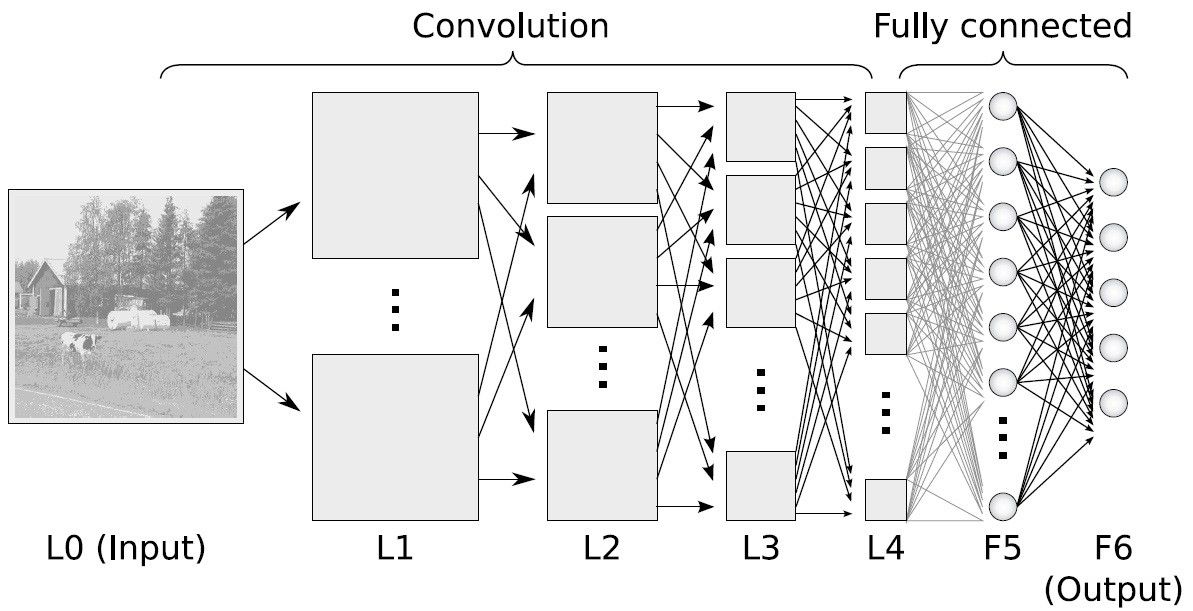
\includegraphics[scale=0.3]{convolutional-neural-network}
      \caption{An example of a convolutional neural network \cite{convNetPicture}. L stands for layer, the boxes corresponds to two dimensional images (maps) and the circles are perceptrons.}
      \label{fig:convNet}
\end{figure}

With reference to Figure \ref{fig:convNet} let us define some useful notations:\\

\section{Fundamental Equations}

\begin{table}[H]
	\centering
	\begin{tabular}{|p{4cm}| l| l|}
		\hline
		Layer index& $l$& $0\leq l \leq L, \quad l,L \in \mathbb{N}$ \\
		\hline
		The number of images in layer $l$ & $N^{l}$ & $N^{l} \in \mathbb{N}$\\
		\hline
		The $i$:th image in layer $l$ & $\pmb{Y}_i^{(l)}$  & $ 1 \leq i \leq N^{l}$ \\
		\hline
		Activation function of layer $l$ & $\phi^{(l)}$ & $\phi^{(l)} : \mathbb{R} \rightarrow \mathbb{R}$\\		
		\hline
		Set of parameters in layer $l$ & $\Omega^{(l)}$  & $\{\omega_i \in \mathbb{R}\}$\\
		\hline
		Combinator function of image $i$ at coordinate $(x,y)$ in layer $l$ & $z^{(l)}_{i,xy}(\pmb{Y}^{(l-1)}_{1:N^{l-1}}, \Omega^{(l)})$& $z^{(l)}_{i,xy}: (\pmb{Y}^{(l-1)}_{1:N^{l-1}}, \Omega^{(l)}) \rightarrow \mathbb{R}$\\
		\hline
		Image coordinates of image $i$ in layer $l$ & $S^l_i$ & $S^l_i \subset \mathbb{N}$\\
		\hline
		Connected images in layer $l+1$ to map i in layer l& $C^l_i$& $C^l_i \subset \mathbb{N}$ \\
		\hline
		 Connected images in layer $l$-$1$ to map $i$ in layer $l$& $D_i^l$& $D^l_i \subset \mathbb{N}$\\
		 \hline
	\end{tabular}
	\caption{Definitions and notations}
	\label{tab:notations}
\end{table}
The network that we will work with in this paper is given by:
\begin{equation}
[\pmb{Y}_i^{(l)}]_{xy} = \phi^{(l)}([\pmb{Z}^{(l)}_{i}(\pmb{Y}^{(l-1)}_{1:N^{l-1}}, \Omega^{(l)})]_{xy})
\label{eq:abstractNetwork}
\end{equation}

Eq. \ref{eq:abstractNetwork} is very abstract and it supports different image sizes, arbitrary connections, shared parameters between units and even images that has random indexing. By deriving the gradient of this equation using back-propagation, we get a very general expression for all kinds of feed-forward networks. Observe that it can be easily expanded to indexing in any dimension, just by replacing $(x,y)$.\\

Let us now consider a set of training data $T = \{(\pmb{Y}_{1:N^{0}}^{(0)}, \pmb{T}_{1:N^L})_t,  1 \leq t \leq N^T \}$. By defining an appropriate error function $r_t : (\pmb{Y}_{1:N^L}^{(L)}, \pmb{T}_{1:N^L})_t \rightarrow \mathbb{R}$ we may now try to minimize the total error by adjusting the parameters of the layers $\Omega^{(l)}$
\begin{equation}
E = \sum_{t = 1}^{N^T}r_t(\pmb{Y}_{1:N^L}^{(L)}, \pmb{T}_{1:N^L})_t
\end{equation}

From here on, we will omit the subscript $t$ since it will only complicate the notation. For batches one may just add $t$ onto all of the below variables and sum it. Observe that the notation $\Omega^{(k)}_m$ means the variable $m$ in the set of parameters $\Omega^{(k)}$.

\begin{gather}
\frac{\partial r}{\partial \Omega^{(k)}_m} = \sum_{i = 1}^{N^L}\sum_{(x,y) \in S^L_i} \frac{\partial r}{\partial [\pmb{Y}^{(L)}_i]_{xy}} \frac{\partial [\pmb{Y}^{(L)}_i]_{xy}}{\partial \Omega^{(k)}_m} \\
\frac{\partial [\pmb{Y}^{(L)}_i]_{xy}}{\partial \Omega^{(k)}_m} = \phi^{(L)'}([\pmb{Z}^{(L)}_{i}]_{xy}) \sum_{j = 1}^{N^{L-1}}\sum_{(x_1,y_1) \in S^{L-1}_j}\frac{\partial [\pmb{Z}^{(L)}_{i}]_{xy}}{\partial [\pmb{Y}^{(L-1)}_j]_{x_1y_1}}\frac{\partial [\pmb{Y}^{(L-1)}_i]_{x_1y_1}}{\partial \Omega^{(k)}_m}
\end{gather}

In general we have the following relation between any two layers $\neq L$:
\begin{equation}
\frac{\partial [\pmb{Y}^{(l)}_i]_{xy}}{\partial \Omega^{(k)}_m} = \phi^{(l)'}([\pmb{Z}^{(l)}_{i}]_{xy}) \sum_{j = 1}^{N^{l-1}}\sum_{(x_1,y_1) \in S^{l-1}_j}\frac{\partial [\pmb{Z}^{(l)}_{i}]_{xy}}{\partial [\pmb{Y}^{(l-1)}_j]_{x_1y_1}}\frac{\partial [\pmb{Y}^{(l-1)}_j]_{x_1y_1}}{\partial \Omega^{(k)}_m}
\end{equation}
From this we can define deltas that will simplify the gradient calculation.
\begin{equation}
[\pmb{\delta}_i^{(L)}]_{xy} = \frac{\partial r}{\partial [\pmb{Y}^{(L)}_i]_{xy}}\phi^{(L)'}([\pmb{Z}^{(L)}_{i}]_{xy})
\label{eq:fundamentalDeltaL}
\end{equation}
\begin{equation}
[\pmb{\delta}_j^{(l)}]_{xy} = \sum_{i = 1}^{N^{l+1}}\sum_{(x_1,y_1) \in S^{l+1}_i} [\pmb{\delta}^{(l+1)}_i]_{x_1y_1} \frac{\partial [\pmb{Z}^{(l + 1)}_{i}]_{x_1y_1}}{\partial [\pmb{Y}^{(l)}_j]_{xy}} \phi^{(l)'}([\pmb{Z}^{(l)}_{j}]_{xy})
\label{eq:fundamentalDelta}
\end{equation}

Finally, the gradient is given by:
\begin{equation}
\frac{\partial r}{\partial \Omega^{(k)}_m} = \sum_{i = 1}^{N^{k}}\sum_{(x,y) \in S^{k}_i} [\pmb{\delta}_i^{(k)}]_{xy} \frac{\partial [\pmb{Z}^{(k)}_i]_{xy}}{\partial \Omega^{(k)}_m}
\label{eq:fundamentalWeight}
\end{equation}

I call Eq. \ref{eq:abstractNetwork}, \ref{eq:fundamentalDeltaL}, \ref{eq:fundamentalDelta}, \ref{eq:fundamentalWeight} the fundamental feed-forward network equations since it defines the gradient and feed-forward relations of any known feed-forward network (known to the Author).

\subsection{MLP}

Let us recap the fundamental equations:
\begin{equation}
[\pmb{Y}_i^{(l)}]_{xy} = \phi^{(l)}([\pmb{Z}^{(l)}_{i}(\pmb{Y}^{(l-1)}_{1:N^{l-1}}, \Omega^{(l)})]_{xy})
\end{equation}
\begin{equation}
[\pmb{\delta}_i^{(L)}]_{xy} = \frac{\partial r}{\partial [\pmb{Y}^{(L)}_i]_{xy}}\phi^{(L)'}([\pmb{Z}^{(L)}_{i}]_{xy})
\end{equation}
\begin{equation}
[\pmb{\delta}_j^{(l)}]_{xy} = \sum_{i = 1}^{N^{l+1}}\sum_{(x_1,y_1) \in S^{l+1}_i} [\pmb{\delta}^{(l+1)}_i]_{x_1y_1} \frac{\partial [\pmb{Z}^{(l + 1)}_{i}]_{x_1y_1}}{\partial [\pmb{Y}^{(l)}_j]_{xy}} \phi^{(l)'}([\pmb{Z}^{(l)}_{j}]_{xy})
\end{equation}
\begin{equation}
\frac{\partial r}{\partial \Omega^{(k)}_m} = \sum_{i = 1}^{N^{k}}\sum_{(x,y) \in S^{k}_i} [\pmb{\delta}_i^{(k)}]_{xy} \frac{\partial [\pmb{Z}^{(k)}_i]_{xy}}{\partial \Omega^{(k)}_m}
\end{equation}

For a fully connected layer such as MLP, we always have the possibility to reshape the images $\pmb{Y}_i^{(l)}, \pmb{Y}_j^{(l-1)}$ so that they are equivalent to vectors $\pmb{y}^{(l)}, \pmb{y}^{(l-1)}$. Hence, the coordinate sets $S_i^{l}, S_i^{l-1}$ contains only one coordinate and we may skip the $(x,y)$ notation. We also have $\phi^{(l)}$ acting component-wise on the input. We may therefore simply the fundamental equations to:

\begin{equation}
y_i^{(l)} = \phi^{(l)}(z^{(l)}_{i}(y^{(l-1)}_{1:N^{l-1}}, \Omega^{(l)}))
\end{equation}
\begin{equation}
\delta_i^{(L)} = \frac{\partial r}{\partial y^{(L)}_i}\phi^{(L)'}(z^{(L)}_{i})
\end{equation}
\begin{equation}
\delta_j^{(l)} = \sum_{i = 1}^{N^{l+1}} \delta^{(l+1)}_i \frac{\partial z^{(l + 1)}_{i}}{\partial y^{(l)}_j} \phi^{(l)'}(z^{(l)}_{j})
\end{equation}
\begin{equation}
\frac{\partial r}{\partial \Omega^{(k)}_m} = \sum_{i = 1}^{N^{k}}\delta_i^{(k)} \frac{\partial z^{(k)}_i}{\partial \Omega^{(k)}_m}
\end{equation}

Let us define $z^{(l)}_i$ by it's vector form:
\begin{equation}
\pmb{z}^{(l)} = \pmb{W}^{(l)}\pmb{y}^{(l-1)} + \pmb{b}^{(l)}
\label{eq:mlp}
\end{equation}
Where $\pmb{Y}^{(l-1)}_{1:N^{l-1}} = \pmb{y}^{(l-1)}$ and $\Omega^{(l)} = \{\pmb{W}^{(l)}, \pmb{b}^{(l)} \}$. By looking at Eq. \ref{eq:mlp} component-wise we obtain the familiar form:
\begin{equation}
y_i^{(l)} = \phi^{(l)}(\sum_{j = 1}^{N^{l-1}}\omega_{ij}^{(l)} y_j^{(l-1)} + b^{(l)}_i)
\end{equation}
Which does indeed to look very similar to the component-wise Eq. \ref{eq:abstractNetwork}.\\
In vector form we have 
\begin{equation}
\pmb{y}^{(l)} = \phi^{(l)}(\pmb{W}^{(l)}\pmb{y}^{(l-1)} + \pmb{b}^{(l)})
\end{equation}

Let us now look at the remaining fundamental equations. We will look at two different output activations and derive the corresponding fundamental equations for this case. First with MSE and linear output which is useful when training a network for regression.
\begin{gather}
\phi^{(L)}(x) = x\\
r(\pmb{t},\pmb{y}^{(L)}) =\frac{1}{2} \| \pmb{t} - \pmb{y}^{(L)} \|^2
\label{eq:MLP_SSE_LINEAR}
\end{gather}
The fundamental equation for the output now transforms into
\begin{equation}
\delta_i^{(L)} =\frac{1}{2} \frac{\partial \| \pmb{t} - \pmb{y}^{(L)} \|^2}{\partial y_i^{(L)}} = -(t_i - y_i^{(L)})
\end{equation}
In vector notation
\begin{equation}
\pmb{\delta}^{(L)} = - (\pmb{t} - \pmb{y}^{(L)})
\end{equation}

We will now consider a cross-entropy error function with soft-max activation. The problem is this case is that the activation function $\phi^{(l)}$ doesnt depend on the other inputs which is necessary for softmax activation. We will therefore set $\phi^{(L)}$ to the identity transform and write the output in terms of $\pmb{Z}_i^{L}(\pmb{Y}_{1:N^L}^L, \Omega^{(L)})$ which can take any type of shape needed.
\begin{gather}
\phi^{(L)}(x) = x\\
z^L_i = \frac{\exp\{ \sum_{j = 1}^{N^{L-1}}\omega_{ij}^{(L)} y_j^{(L-1)} + b^{(L)}_i\}}{\sum_{k = 1}^{N^L} \exp\{\sum_{j = 1}^{N^{L-1}}\omega_{kj}^{(L)} y_j^{(L-1)} + b^{(L)}_k\}}
\end{gather}
For a single binary classification task, the Cross-entropy function takes the form:
\begin{equation}
r(\pmb{t}, \pmb{y}^{(L)}) = -(t \log(y^{(L)}) + (1 - t)\log(1 - y^{(L)}))
\end{equation} 
Which also implies that we need to use a normal Sigmoid activation instead of the Softmax activation function. For multiple classes the CE function is given by
\begin{equation}
r(\pmb{t}, \pmb{y}^{(L)}) = - \sum_{i = 0}^{N^L} t_i \log{y^{(L)}_i}
\end{equation}
Let us now calculate the delta at the output layer for this case.
\begin{gather}
\delta_i^{(L)} =-\frac{\partial\sum_{j = 0}^{N^L} t_j \log{y^{(L)}_j}}{\partial y_i^{L}} = -\frac{t_i}{y_i^{(L)}}\\
\end{gather} 
However, with this change in $z_i^{(L)}$ extra care has to be taken to the derivative $\frac{\partial z_i^{(L)}}{\partial y_j^{(L-1)}}$. It can be shown that
\begin{equation}
\delta_i^{(L)}\frac{\partial z_i^{(L)}}{\partial y_j^{(L-1)}} = -(t_i - y_i^{(L)})\omega_{ij}^{(L)}
\end{equation}

In any case, with one dimensional sigmoid and CE, softmax with CE and regression with linear equations. We obtain exactly the same update equations.

\begin{remark}
	Note that $\delta_i^{(L)}$ in the case of a one dimensional variable with sigmoid $\phi^{(L)}$ we obtain the same equations as in the regression case. I.e. $\delta^{(L)} = -(t - y^{(L)})$.
\end{remark}

A case that will not give the same update equations is if we use the MLE norm together with a non-trivial activation function at layer $L$.
\begin{equation}
\delta_i^{(L)} =\frac{1}{2} \frac{\partial \| \pmb{t} - \pmb{y}^{(L)} \|^2}{\partial y_i^{(L)}} = -(t_i - y_i^{(L)}) \phi^{'(L)}(z_i^{(L)})
\end{equation}
This may also be expanded to the CE function if you carefully choose the output activation function $\phi^{(L)}(z_i^{(L)})$ so that it has positive or zero values.
\begin{equation}
\delta_i^{(L)} = -\frac{t_i - y_i^{(L)}}{y^{(L)}_i(1 - y^{(L)}_i)} \phi^{'(L)}(z_i^{(L)})
\end{equation}


For a layer not equal to the output layer, we have the following expression (where the activation function is normally a tanh or a sigmoid.)
\begin{gather}
z_i^{(l)} = \sum_{j = 1}^{N^{l-1}}\omega_{ij}^{(l)} y_j^{(l-1)} + b^{(l)}_i \\
\delta^{(l)}_i = \sum_{j = 1}^{N^{l + 1}}\omega_{ji}^{(l+1)} \delta_j^{(l+1)}\phi^{'(l)}(z_i^{(l)})
\end{gather}
Or in vector notation
\begin{equation}
\pmb{\delta}^{(l)} = \pmb{W}^{(l+1)T} \pmb{\delta}^{(l+1)} \circ \phi^{'(l)}(\pmb{z}^{(l)})
\end{equation}

Before ending this section, let us finish by calculating the gradient of this layer
\begin{equation}
\frac{\partial r}{\partial \Omega^{(l)}_m} = \sum_{i = 1}^{N^{l}}\delta_j^{(l)} \frac{\partial z^{(l)}_i}{\partial \Omega^{(l)}_m}
\end{equation}

\begin{equation}
\frac{\partial r}{\partial \omega^{(l)}_{kj}} = \sum_{i = 1}^{N^{l}}\delta_j^{(l)} \frac{\partial \sum_{m = 1}^{N^{l-1}}\omega_{im}^{(l)} y_m^{(l-1)} + b^{(l)}_i}{\partial \omega^{(l)}_{kj}}
\end{equation}
\begin{equation}
\frac{\partial r}{\partial \omega^{(l)}_{kj}} = \delta_k^{(l)}y_j^{(l-1)}
\end{equation}
\begin{equation}
\frac{\partial r}{\partial b^{(l)}_{k}} = \delta_k^{(l)}
\end{equation}

In vector form
\begin{equation}
\Delta\pmb{W}^{(l)} = \pmb{\delta}^{(l)} \pmb{y}^{(l-1)T}
\end{equation}
\begin{equation}
\Delta \pmb{b}^{(l)} = \pmb{\delta}^{(l)}
\end{equation}

The important equations are summarized in the below tables:

\begin{table}[H]
	\centering
	\begin{tabular}{|p{4cm}| l|}
		\hline
		Error function & $r(\pmb{t}, \pmb{y}^{(L)})$ \\
		\hline
		CE, binary& $-(t \log(y^{(L)}) + (1 - t)\log(1 - y^{(L)}))$\\
		\hline
		CE, multiple classes& $- \sum_{i = 0}^{N^L} t_i \log{y^{(L)}_i}$\\
		\hline
		MSE & $\frac{1}{2} \| \pmb{t} - \pmb{y}^{(L)} \|^2$\\
		\hline
	\end{tabular}
	\caption{Common error functions.}
\end{table}

\begin{table}[H]
	\centering
	\begin{tabular}{|p{4cm}| l|}
		\hline
		(Error, Activation) & $\pmb{\delta}^{(L)}$ \\
		\hline
		(CE, Softmax) & $- (\pmb{t} - \pmb{y}^{(L)})$ \\
		\hline
		(CE - binary, Sigmoid) & $- (t - y^{(L)})$ \\
		\hline
		(MSE, Linear) & $- (\pmb{t} - \pmb{y}^{(L)})$ \\
		\hline
		(MSE, Any) & $ -(\pmb{t}_i - \pmb{y}_i^{(L)}) \circ \phi^{'(L)}(\pmb{z}_i^{(L)})$ \\
		\hline
		(CE, Any) & $- \pmb{t} \circ \frac{1}{\pmb{y}^{(L)}}\circ \phi^{'(L)}(\pmb{z}_i^{(L)})$ \\
		\hline
		(CE - binary, Any) & $-\frac{t - y^{(L)}}{y^{(L)}(1 - y^{(L)})} \phi^{'(L)}(z^{(L)})$ \\
		\hline			
	\end{tabular}
	\label{tab:outputDeltaMLP}
	\caption{Output deltas for different activations and error functions.}
\end{table}

\begin{table}[H]
	\centering
	\begin{tabular}{|p{4cm}| l|}
		\hline
		Feed forward  & $\pmb{z}^{(l)} = \pmb{W}^{(l)}\pmb{y}^{(l-1)} + \pmb{b}^{(l)}$ \\
		\hline
		Feed forward & $\pmb{y}^{(l)} = \phi^{(l)}(\pmb{z}^{(l)})$\\
		\hline
		Back propagation & $\pmb{\delta}^{(L)}$ by Table \ref{tab:outputDeltaMLP}\\
		\hline
		Back propagation & $\pmb{\delta}^{(l)} = \pmb{W}^{(l+1)T} \pmb{\delta}^{(l+1)} \circ \phi^{'(l)}(\pmb{z}^{(l)})$\\
		\hline
		Weight update & $\Delta\pmb{W}^{(l)} = \pmb{\delta}^{(l)} \pmb{y}^{(l-1)T}$\\
		\hline
		Bias update & $\Delta \pmb{b}^{(l)} = \pmb{\delta}^{(l)}$\\
		\hline
	\end{tabular}
	\caption{Fundamental MLP equations.}
\end{table}

\subsection{Radial basis layer}
Let use once again recall the fundamental equations.
\begin{equation}
[\pmb{Y}_i^{(l)}]_{xy} = \phi^{(l)}([\pmb{Z}^{(l)}_{i}(\pmb{Y}^{(l-1)}_{1:N^{l-1}}, \Omega^{(l)})]_{xy})
\end{equation}
\begin{equation}
[\pmb{\delta}_i^{(L)}]_{xy} = \frac{\partial r}{\partial [\pmb{Y}^{(L)}_i]_{xy}}\phi^{(L)'}([\pmb{Z}^{(L)}_{i}]_{xy})
\end{equation}
\begin{equation}
[\pmb{\delta}_j^{(l)}]_{xy} = \sum_{i = 1}^{N^{l+1}}\sum_{(x_1,y_1) \in S^{l+1}_i} [\pmb{\delta}^{(l+1)}_i]_{x_1y_1} \frac{\partial [\pmb{Z}^{(l + 1)}_{i}]_{x_1y_1}}{\partial [\pmb{Y}^{(l)}_j]_{xy}} \phi^{(l)'}([\pmb{Z}^{(l)}_{j}]_{xy})
\end{equation}
\begin{equation}
\frac{\partial r}{\partial \Omega^{(k)}_m} = \sum_{i = 1}^{N^{k}}\sum_{(x,y) \in S^{k}_i} [\pmb{\delta}_i^{(k)}]_{xy} \frac{\partial [\pmb{Z}^{(k)}_i]_{xy}}{\partial \Omega^{(k)}_m}
\end{equation}

Once again as for the MLP, if we have image inputs we may always reshape the maps into vectors. We may therefore omit the subscript $(x,y)$. Yielding the below fundamental equations:
\begin{equation}
y_i^{(l)} = \phi^{(l)}(z^{(l)}_{i}(y^{(l-1)}_{1:N^{l-1}}, \Omega^{(l)}))
\end{equation}
\begin{equation}
\delta_i^{(L)} = \frac{\partial r}{\partial y^{(L)}_i}\phi^{(L)'}(z^{(L)}_{i})
\end{equation}
\begin{equation}
\delta_j^{(l)} = \sum_{i = 1}^{N^{l+1}} \delta^{(l+1)}_i \frac{\partial z^{(l + 1)}_{i}}{\partial y^{(l)}_j} \phi^{(l)'}(z^{(l)}_{j})
\end{equation}
\begin{equation}
\frac{\partial r}{\partial \Omega^{(k)}_m} = \sum_{i = 1}^{N^{k}}\delta_i^{(k)} \frac{\partial z^{(k)}_i}{\partial \Omega^{(k)}_m}
\end{equation}

For a radial basis function, the activation doesn't really make sense to use the separation between activation and combinator function. We will thus always regard $\phi^{(l)}(x) = x$ as the identity map. We may therefore simplify the fundamental equations further.
\begin{equation}
y_i^{(l)} = z^{(l)}_{i}(y^{(l-1)}_{1:N^{l-1}}, \Omega^{(l)})
\end{equation}
\begin{equation}
\delta_i^{(L)} = \frac{\partial r}{\partial y^{(L)}_i}
\end{equation}
\begin{equation}
\delta_j^{(l)} = \sum_{i = 1}^{N^{l+1}} \delta^{(l+1)}_i \frac{\partial z^{(l + 1)}_{i}}{\partial y^{(l)}_j}
\end{equation}
\begin{equation}
\frac{\partial r}{\partial \Omega^{(k)}_m} = \sum_{i = 1}^{N^{k}}\delta_i^{(k)} \frac{\partial z^{(k)}_i}{\partial \Omega^{(k)}_m}
\end{equation}

For a general radial basis layer, we usually set\\ $z^{(l)}_{i}(y^{(l-1)}_{1:N^{l-1}}, \Omega^{(l)}) = \rho(\|y^{(l-1)}_{1:N^{l-1}} - \pmb{c}_i^{(l)}\|)$. Which in practice normally looks like: 
\begin{equation}
z^{(l)}_{i}(y^{(l-1)}_{1:N^{l-1}}, \Omega^{(l)}) = \exp\{ -\beta_i\|y^{(l-1)}_{1:N^{l-1}} - \pmb{c}_i^{(l)}\| \}
\end{equation}

The parameter set thus consists of $\Omega^{(l)} = \{(\pmb{c}_i^{(l)}, \beta_i) \}$. If one is interested in using RBF:s as outputs, a common approach is to linearly combine the RBF:s at the output layer. This in turn may be viewed as
\begin{equation}
z^{(L)}_{i}(y^{(L-1)}_{1:N^{L-1}}, \Omega^{(L)}) = \sum_{j \in D^{L}_i} a_{ij} \rho(\|y^{(l-1)}_{1:N^{l-1}} - \pmb{c}_i^{(l)}\|)
\end{equation}
Where $D^{L}_i$ is as indicated in the notation's table. The connected images to the node $i$. Normally, it's fully connected. The parameter set of the last layer is thus $\Omega^{(l)} = \{a_{ij} \}$.

\subsection{Convolution Layer}

As usual, always start with the fundamental equations:
\begin{equation}
[\pmb{Y}_i^{(l)}]_{xy} = \phi^{(l)}([\pmb{Z}^{(l)}_{i}(\pmb{Y}^{(l-1)}_{1:N^{l-1}}, \Omega^{(l)})]_{xy})
\end{equation}
\begin{equation}
[\pmb{\delta}_i^{(L)}]_{xy} = \frac{\partial r}{\partial [\pmb{Y}^{(L)}_i]_{xy}}\phi^{(L)'}([\pmb{Z}^{(L)}_{i}]_{xy})
\end{equation}
\begin{equation}
[\pmb{\delta}_j^{(l)}]_{xy} = \sum_{i = 1}^{N^{l+1}}\sum_{(x_1,y_1) \in S^{l+1}_i} [\pmb{\delta}^{(l+1)}_i]_{x_1y_1} \frac{\partial [\pmb{Z}^{(l + 1)}_{i}]_{x_1y_1}}{\partial [\pmb{Y}^{(l)}_j]_{xy}} \phi^{(l)'}([\pmb{Z}^{(l)}_{j}]_{xy})
\end{equation}
\begin{equation}
\frac{\partial r}{\partial \Omega^{(k)}_m} = \sum_{i = 1}^{N^{k}}\sum_{(x,y) \in S^{k}_i} [\pmb{\delta}_i^{(k)}]_{xy} \frac{\partial [\pmb{Z}^{(k)}_i]_{xy}}{\partial \Omega^{(k)}_m}
\end{equation}

This is the first time that the coordinates will come in handy. Observe however that we will omit the residual equations (i.e. $[\pmb{\delta}_i^{(L)}]_{xy}$) for a convolutional layer since it will not be used immediately. However, it is very straight-forward to derive for an interested reader.\\

Let us start off by defining
\begin{equation}
[\pmb{Z}^{(l)}_{i}(\pmb{Y}^{(l-1)}_{1:N^{l-1}}, \Omega^{(l)})]_{xy} = \sum_{j \in D_i^{l}} (\pmb{Y}_j^{(l-1)} \star \pmb{\omega}_{ij}^{(l)})(x,y) + b^{(l)}_i
\end{equation}
\begin{equation}
(\pmb{Y}_j^{(l-1)} \star \pmb{\omega}_{ij}^{(l)})(x,y) = \sum_{u = 0}^{M_u} \sum_{v = 0}^{M_v} [\pmb{Y}_j^{(l-1)}]_{x + u, y + v} \cdot [\pmb{\omega}_{ij}^{(l)}]_{u,v}
\end{equation}
Where $M_u, M_v$ is the width and height of the kernel $\pmb{\omega}_{ij}^{(l)}$. Furthermore, we have the parameters $\Omega^{(l)} = \{\pmb{\omega}_{ij}^{(l)}, \pmb{b}^{(l)} \}$.
\begin{remark}
	Observe that in most cases $\pmb{\omega}_{ij}^{(l)} = \pmb{\omega}_{i}^{(l)}$
\end{remark}
\begin{remark}
	Observe that there's nothing limiting us at the moment to use different sizes of the kernels in the same layer. However, practically this is rarely used.
\end{remark}
\begin{remark}
	In practical applications where sub-sampling is used, one may in some cases simply sub-sample by taking every $k$:th coordinate in the x,y directions. Instead of convolving the entire image and then sub-sample every $k$:th pixel, we may put the sub-sampling operation directly in the convolution operation. Thus yielding:
	\begin{equation}
	(\pmb{Y}_j^{(l-1)} \star \pmb{\omega}_{ij}^{(l)})(x,y) = \sum_{u = 0}^{M_u} \sum_{v = 0}^{M_v} [\pmb{Y}_j^{(l-1)}]_{kx + u, ky + v} \cdot [\pmb{\omega}_{ij}^{(l)}]_{u,v}
	\end{equation}
	\label{remark:convolutionSubSamping}
\end{remark}

We will now turn to the interesting part of the convolutional layer. That is, how do we calculate the deltas? 

\begin{gather}
\frac{\partial [\pmb{Z}^{(l + 1)}_{i}(\pmb{Y}^{(l)}_{1:N^{l-1}}, \Omega^{(l + 1)})]_{xy}}{\partial [\pmb{Y}^{(l)}_j]_{x_1y_1}} = \frac{\partial \sum_{k \in D_i^{l+1}} (\pmb{Y}_k^{(l)} \star \pmb{\omega}_{ik}^{(l + 1)})(x,y) + b^{(l)}_i}{\partial [\pmb{Y}^{(l)}_j]_{x_1y_1}} =\\
\frac{\partial \sum_{u = 0}^{M_u} \sum_{v = 0}^{M_v} [\pmb{Y}_j^{(l)}]_{x + u, y + v} \cdot [\pmb{\omega}_{ij}^{(l + 1)}]_{u,v}}{\partial [\pmb{Y}^{(l)}_j]_{x_1y_1}} \mathds{1}_{\{j \in D^{l+1}_i\}} = \\
\sum_{u = 0}^{M_u} \sum_{v = 0}^{M_v} \mathds{1}_{\{x_1 = x + u, y_1 = y + v\}} \cdot [\pmb{\omega}_{ij}^{(l+1)}]_{u,v}\mathds{1}_{\{j \in D^{l+1}_i\}}
\end{gather}
This latest function is pretty hard to get an intuition from on its own. Therefore, let us put it into the right context.

\begin{equation}
[\pmb{\delta}_j^{(l)}]_{xy} = \sum_{i = 1}^{N^{l+1}}\sum_{(x_1,y_1) \in S^{l+1}_i} [\pmb{\delta}^{(l+1)}_i]_{x_1y_1} \frac{\partial [\pmb{Z}^{(l + 1)}_{i}]_{x_1y_1}}{\partial [\pmb{Y}^{(l)}_j]_{xy}} \phi^{(l)'}([\pmb{Z}^{(l)}_{j}]_{xy})
\end{equation}
\begin{gather}
[\pmb{\delta}_j^{(l)}]_{xy} = \\
\sum_{i = 1}^{N^{l+1}}\sum_{(x_1,y_1) \in S^{l+1}_i} [\pmb{\delta}^{(l+1)}_i]_{x_1y_1} \sum_{u = 0}^{M_u} \sum_{v = 0}^{M_v} \mathds{1}_{\{x = x_1 + u, y = y_1 + v\}} \cdot [\pmb{\omega}_{ij}^{(l+1)}]_{u,v}\mathds{1}_{\{j \in D^{l+1}_i\}} \phi^{(l)'}([\pmb{Z}^{(l)}_{j}]_{xy})
\label{eq:horrible}
\end{gather}
The above expression looks horrible, so let us take some time to analyze it.
\begin{equation}
\sum_{(x_1,y_1) \in S^{l+1}_i} [\pmb{\delta}^{(l+1)}_i]_{x_1y_1} \sum_{u = 0}^{M_u} \sum_{v = 0}^{M_v} \mathds{1}_{\{x = x_1 + u, y = y_1 + v\}} \cdot [\pmb{\omega}_{ij}^{(l+1)}]_{u,v}
\label{eq:intermediateConvolution}
\end{equation}
What does this equation really mean? Imagine that we have performed the summation over all $(x_1, y_1)$. The only terms that will survive are the one who's given by $(x = x_1 + u, y = y_1 + v)$. This is true, but one should be careful to perform the variable substitution directly, since we have to observe that $(x,y)$ is defined on $S^l_j$ whereas $(x_1, y_1)$ is defined on $S_i^{l+1}$. By performing the summation and substitute $(x_1 = x-u, y_1 = y-v)$, we may have for some combination of $(x,y,u,v)$ that $(x_1 = x-u, y_1 = y-v) \notin S_i^{l+1}$. Therefore, when performing the summation we have to take this into account. Eq. \ref{eq:intermediateConvolution} is therefore transformed into:
\begin{equation}
\sum_{u = 0}^{M_u} \sum_{v = 0}^{M_v}  [\pmb{\delta}^{(l+1)}_i]_{x - u,y - v}  [\pmb{\omega}_{ij}^{(l+1)}]_{u,v} \mathds{1}_{\{(x - u, y - v) \in S^{l+1}_i\}}
\label{eq:simplifiedIntermediateConvolution}
\end{equation}
If you were a mathematician you would probably already scream about all the omitted details. But above is actually incorrect in the sense that $[\pmb{\delta}^{(l+1)}_i]_{x - u,y - v}$ may not even be defined. But on those values, we kind of indicate that with the $\mathds{1}$ function. So imagine that you expand the size of $\pmb{\delta}^{(l+1)}_i$ if you want to be rigorous.\\

Let us now turn to the implementor's perspective. A very simple method of not hassling with the boundaries is to allow expansion of $\pmb{\delta}^{(l+1)}_i$ so that we have zeros located on the coordinates where $\mathds{1}_{\{(x - u, y - v) \in S^{l+1}_i\}}$ doesn't hold. Let us denote this delta by $\tilde{\pmb{\delta}}^{(l+1)}_i$. And we obtain
\begin{equation}
\sum_{u = 0}^{M_u} \sum_{v = 0}^{M_v}  [\tilde{\pmb{\delta}}^{(l+1)}_i]_{x - u,y - v}  [\pmb{\omega}_{ij}^{(l+1)}]_{u,v}
\label{eq:negativeConvolution}
\end{equation}    

Furthermore, we observe that convolution defined by \ref{eq:negativeConvolution} is actually equivalent to convolution previously defined by simply rotating the kernel $\pmb{\omega}_{ij}^{(l+1)}$ by 180 degrees. Let us denote this kernel by $\tilde{\pmb{\omega}}_{ij}^{(l+1)}$.
\begin{equation}
\sum_{u = 0}^{M_u} \sum_{v = 0}^{M_v}  [\tilde{\pmb{\delta}}^{(l+1)}_i]_{x - u,y - v}  [\pmb{\omega}_{ij}^{(l+1)}]_{u,v} = (\tilde{\pmb{\delta}}^{(l+1)}_i \star \tilde{\pmb{\omega}}_{ik}^{(l + 1)})(x,y)
\end{equation}
Eq. \ref{eq:horrible} is now simplified to:

\begin{equation}
[\pmb{\delta}_j^{(l)}]_{xy} =\sum_{i = 1}^{N^{l+1}}(\tilde{\pmb{\delta}}^{(l+1)}_i \star \tilde{\pmb{\omega}}_{ij}^{(l + 1)})(x,y)\mathds{1}_{\{j \in D^{l+1}_i\}} \phi^{(l)'}([\pmb{Z}^{(l)}_{j}]_{xy})
\label{eq:convolutionDeltaNeedsSimplification}
\end{equation}
By noting that $\sum_{i = 1}^{N^{l+1}}\mathds{1}_{\{j \in D^{l+1}_i\}}$ is actually equivalent to all connected images from $j$ in $l$ to $l+1$. Eq. \ref{eq:convolutionDeltaNeedsSimplification} is therefore transformed into:
\begin{equation}
[\pmb{\delta}_j^{(l)}]_{xy} =\sum_{i \in C^l_j}(\tilde{\pmb{\delta}}^{(l+1)}_i \star \tilde{\pmb{\omega}}_{ij}^{(l + 1)})(x,y)\phi^{(l)'}([\pmb{Z}^{(l)}_{j}]_{xy})
\label{eq:convolutionDeltaSimplified}
\end{equation}

\begin{remark}
	Let us continue on Remark \ref{remark:convolutionSubSamping} which optimizes a combined convolution and sub-sampling operation by doing it simultaneously. In this case Eq. \ref{eq:intermediateConvolution} takes the form
	\begin{equation}
	\sum_{(x_1,y_1) \in S^{l+1}_i} [\pmb{\delta}^{(l+1)}_i]_{x_1y_1} \sum_{u = 0}^{M_u} \sum_{v = 0}^{M_v} \mathds{1}_{\{x = kx_1 + u, y = ky_1 + v\}} \cdot [\pmb{\omega}_{ij}^{(l+1)}]_{u,v}
	\label{eq:intermediateConvolutionSubSampling}
	\end{equation}
	The coordinate change is not as straight forward in this case since we are dealing with integer equations and they may not be directly divided. However, this case can be handled rather neatly just by using vanilla sub-sampling and discard calculating unnecessary coordinates.
	
\end{remark}

Lastly, let us now derive the equations for weight updates.

\begin{equation}
\frac{\partial r}{\partial [\pmb{\omega}_{pq}^{(l)}]_{u,v}} = \sum_{i = 1}^{N^{l}}\sum_{(x,y) \in S^{l}_i} [\pmb{\delta}_i^{(l)}]_{xy} \frac{\partial [\pmb{Z}^{(l)}_i]_{xy}}{\partial [\pmb{\omega}_{pq}^{(l)}]_{u,v}}
\label{eq:weightConv}
\end{equation}
\begin{equation}
[\pmb{Z}^{(k)}_i]_{xy} = \sum_{j \in D_i^{l}} \sum_{m = 0}^{M_u} \sum_{n = 0}^{M_v} [\pmb{Y}_j^{(l-1)}]_{x + m, y + n} \cdot [\pmb{\omega}_{ij}^{(l)}]_{m,n} + b^{(l)}_i
\label{eq:zConv}
\end{equation}
By inserting Eq. \ref{eq:zConv} in Eq. \ref{eq:weightConv}. We obtain
\begin{equation}
\frac{\partial r}{\partial [\pmb{\omega}_{pq}^{(l)}]_{u,v}} = \sum_{i = 1}^{N^{l}}\sum_{(x,y) \in S^{l}_i} [\pmb{\delta}_i^{(l)}]_{xy} \sum_{j \in D_i^{l}} \sum_{m = 0}^{M_u} \sum_{n = 0}^{M_v} [\pmb{Y}_j^{(l-1)}]_{x + m, y + n} \cdot \frac{\partial[\pmb{\omega}_{ij}^{(l)}]_{m,n}}{\partial[\pmb{\omega}_{pq}^{(l)}]_{u,v}}
\end{equation}
As before,  $\sum_{i = 1}^{N^{l+1}}\mathds{1}_{\{j \in D^{l+1}_i\}}$ is equivalent to all connected images from $j$ in $l$ to $l+1$.

\begin{equation}
\frac{\partial r}{\partial [\pmb{\omega}_{pq}^{(l)}]_{u,v}} = \sum_{(x,y) \in S^{l}_p}[\pmb{\delta}_p^{(l)}]_{xy} [\pmb{Y}_q^{(l-1)}]_{x + u, y + v}
\end{equation}
And for the more common case where we don't distinguish the kernel between the connections, we obtain
\begin{equation}
\frac{\partial r}{\partial [\pmb{\omega}_{i}^{(l)}]_{u,v}} = \sum_{(x,y) \in S^{l}_i} \sum_{j \in C^{l}_i}[\pmb{\delta}_i^{(l)}]_{xy} [\pmb{Y}_j^{(l-1)}]_{x + u, y + v}
\end{equation}
For the bias we obtain
\begin{equation}
\frac{\partial r}{\partial b^{(l)}_i} =  \sum_{(x,y) \in S^{l}_i}  [\pmb{\delta}_i^{(l)}]_{xy}
\end{equation}

Let us now recap all the important equations.
\begin{table}[H]
	\centering
	\begin{tabular}{|p{4cm}| p{8cm}|}
		\hline
		Convolution Definition & $(\pmb{Y}_j^{(l-1)} \star \pmb{\omega}_{ij}^{(l)})(x,y) = \sum_{u = 0}^{M_u} \sum_{v = 0}^{M_v} [\pmb{Y}_j^{(l-1)}]_{x + u, y + v} \cdot [\pmb{\omega}_{ij}^{(l)}]_{u,v}$ \\
		\hline
		Feed forward  & $[\pmb{Y}^{(l)}_i]_{xy} =  \phi^{(l)} (\sum_{j \in D_i^{l}} (\pmb{Y}_j^{(l-1)} \star \pmb{\omega}_{ij}^{(l)})(x,y))$ \\
		\hline
		Delta padding & $\tilde{\pmb{\delta}}^{(l+1)}_i$ by padding  $\mathds{1}_{\{(x - u, y - v) \in S^{l+1}_i\}}$, which corresponds to a padding of size $M_u, M_v$ around $\pmb{\delta}_i^{(l+1)}$.\\
		\hline
		Kernel rotation & $\tilde{\pmb{\omega}}_{ij}^{(l+1)} = rot180(\pmb{\omega}_{ij}^{(l+1)})$\\
		\hline 
		Back propagation & $[\pmb{\delta}_j^{(l)}]_{xy} =\sum_{i \in C^l_j}(\tilde{\pmb{\delta}}^{(l+1)}_i \star \tilde{\pmb{\omega}}_{ij}^{(l + 1)})(x,y)\phi^{(l)'}([\pmb{Z}^{(l)}_{j}]_{xy})$\\
		\hline
		Kernel update with multiple kernels per map& $\frac{\partial r}{\partial [\pmb{\omega}_{pq}^{(l)}]_{u,v}} = \sum_{(x,y) \in S^{l}_p}[\pmb{\delta}_p^{(l)}]_{xy} [\pmb{Y}_q^{(l-1)}]_{x + u, y + v}$\\
		\hline
		Kernel update with one kernel per map & $\frac{\partial r}{\partial [\pmb{\omega}_{i}^{(l)}]_{u,v}} = \sum_{(x,y) \in S^{l}_i} \sum_{j \in C^{l}_i}[\pmb{\delta}_i^{(l)}]_{xy} [\pmb{Y}_j^{(l-1)}]_{x + u, y + v}$\\
		\hline
		Bias update & $\frac{\partial r}{\partial b^{(l)}_i} =  \sum_{(x,y) \in S^{l}_i}  [\pmb{\delta}_i^{(l)}]_{xy}$\\
		\hline
	\end{tabular}
	\caption{Fundamental convolution equations.}
\end{table}

\subsection{Pooling and Sub Sampling}

The purpose of performing pooling or sub-sampling is to reduce the dimensionality of the problem.
As usual, always start with the fundamental equations:
\begin{equation}
	[\pmb{Y}_i^{(l)}]_{xy} = \phi^{(l)}([\pmb{Z}^{(l)}_{i}(\pmb{Y}^{(l-1)}_{1:N^{l-1}}, \Omega^{(l)})]_{xy})
\end{equation}
\begin{equation}
	[\pmb{\delta}_i^{(L)}]_{xy} = \frac{\partial r}{\partial [\pmb{Y}^{(L)}_i]_{xy}}\phi^{(L)'}([\pmb{Z}^{(L)}_{i}]_{xy})
\end{equation}
\begin{equation}
	[\pmb{\delta}_j^{(l)}]_{xy} = \sum_{i = 1}^{N^{l+1}}\sum_{(x_1,y_1) \in S^{l+1}_i} [\pmb{\delta}^{(l+1)}_i]_{x_1y_1} \frac{\partial [\pmb{Z}^{(l + 1)}_{i}]_{x_1y_1}}{\partial [\pmb{Y}^{(l)}_j]_{xy}} \phi^{(l)'}([\pmb{Z}^{(l)}_{j}]_{xy})
\end{equation}
\begin{equation}
	\frac{\partial r}{\partial \Omega^{(k)}_m} = \sum_{i = 1}^{N^{k}}\sum_{(x,y) \in S^{k}_i} [\pmb{\delta}_i^{(k)}]_{xy} \frac{\partial [\pmb{Z}^{(k)}_i]_{xy}}{\partial \Omega^{(k)}_m}
\end{equation}

In this section we will consider three types of sub-sampling and pooling layers. Let us start with sub-sampling as defined by LeCun. Also observe that we will not consider the $\pmb{\delta}_i^{(L)}$ since pooling will very rarely be located on the output layer.
\subsubsection{Weighed sub-sampling}
Let us begin by defining the sub-sampling regime.
\begin{equation}
[\pmb{Z}^{(l)}_{i}(\pmb{Y}^{(l-1)}_{1:N^{l-1}}, \Omega^{(l)})]_{xy} = \sum_{j \in D^l_i} \alpha_{ij} \sum_{u = 0}^{K_u - 1}\sum_{v = 0}^{K_v - 1} [\pmb{Y}^{(l-1)}_j]_{xK_u + u, yK_v + v} + b_i^{(l)}
\end{equation}
Where $(K_u, K_v)$ defines the sub-sampling factors in the respective dimensions. Normally they are all equal, but we distinguish them here for generality. One could also allow different sub-sampling sizes between interconnected maps, but the notation becomes rather tedious. Furthermore, we also allow interconnections in the sub-sampling layer. However, in a practical application $j = i$ and the entire scheme gets reduced to
\begin{equation}
[\pmb{Z}^{(l)}_{i}(\pmb{Y}^{(l-1)}_{1:N^{l-1}}, \Omega^{(l)})]_{xy} =  \alpha_{i} \sum_{u = 0}^{K - 1}\sum_{v = 0}^{K - 1} [\pmb{Y}^{(l-1)}_i]_{xK + u, yK + v} + b_i^{(l)}
\end{equation}

The big question now is how to we propagate the delta through this sub-sampling layer. Let us study
\begin{gather}
\frac{\partial [\pmb{Z}^{(l)}_{i}]_{x_1y_1}}{\partial [\pmb{Y}^{(l-1)}_k]_{xy}} = \frac{\partial \sum_{j \in D^l_i} \alpha_{ij} \sum_{u = 0}^{K_u - 1}\sum_{v = 0}^{K_v - 1} [\pmb{Y}^{(l-1)}_j]_{x_1K_u + u, y_1K_v + v} + b_i^{(l)}}{\partial  [\pmb{Y}^{(l-1)}_k]_{xy}} \\
= \alpha_{ik} \sum_{u = 0}^{K_u - 1}\sum_{v = 0}^{K_v - 1} \mathds{1}_{\{x = x_1K_u + u, y = y_1K_v + v\}}\mathds{1}_{\{k \in D^l_i\}}
\end{gather}

Let us now put this into the fundamental equation governing delta, in order to simplify it further.
\begin{equation}
	[\pmb{\delta}_j^{(l)}]_{xy} = \sum_{i = 1}^{N^{l+1}}\sum_{(x_1,y_1) \in S^{l+1}_i} [\pmb{\delta}^{(l+1)}_i]_{x_1y_1} \alpha_{ij} \sum_{u = 0}^{K_u - 1}\sum_{v = 0}^{K_v - 1} \mathds{1}_{\{x = x_1K_u + u, y = y_1K_v + v\}}\mathds{1}_{\{j \in D^{l+1}_i\}} \phi^{(l)'}([\pmb{Z}^{(l)}_{j}]_{xy})
\end{equation}
As noted earlier in the convolution section. The sum $\sum_{i = 1}^{N^{l+1}}\mathds{1}_{\{j \in D^{l+1}_i\}}$, is equivalent to summing $i$ over $C_j^{l}$ instead. Which transforms the expression into
\begin{equation}
	[\pmb{\delta}_j^{(l)}]_{xy} = \sum_{i \in C_j^{l}}\sum_{(x_1,y_1) \in S^{l+1}} [\pmb{\delta}^{(l+1)}_i]_{x_1y_1} \alpha_{ij} \sum_{u = 0}^{K_u - 1}\sum_{v = 0}^{K_v - 1} \mathds{1}_{\{x = x_1K_u + u, y = y_1K_v + v\}} \phi^{(l)'}([\pmb{Z}^{(l)}_{j}]_{xy})
	\label{eq:subSampleDeltaComplex}
\end{equation}
As usual the expressions looks rather horrible, but fear not. For simplicity, we assume the same sizes in the layers because otherwise a lot more subscripts has to be added to the notation. Instead of trying a variable substitution as in the convolution case, we notice here that the summation\\
$\sum_{(x_1,y_1) \in S^{l+1}}\sum_{u = 0}^{K_u - 1}\sum_{v = 0}^{K_v - 1}\mathds{1}_{\{x = x_1K_u + u, y = y_1K_v + v\}}$ will correspond to the entire image of the previous layer since we don't allow overlapping. Concretely this means that we will have the value $[\pmb{\delta}^{(l+1)}_i]_{x_1y_1}$ on sub rectangles defined on $\sum_{u = 0}^{K_u - 1}\sum_{v = 0}^{K_v - 1}\mathds{1}_{\{x_1K_u + u, y_1K_v + v\}}$. This important insight can simplify Eq. \ref{eq:subSampleDeltaComplex} into
\begin{equation}
[\pmb{\delta}_j^{(l)}]_{xy} = \sum_{i \in C_j^{l}} \alpha_{ij}[\pmb{\delta}^{(l+1)}_i]_{\lfloor \frac{x}{K_u}\rfloor, \lfloor \frac{y}{K_v} \rfloor} \phi^{(l)'}([\pmb{Z}^{(l)}_{j}]_{xy})
\end{equation}
And of course, for the practical situations the delta transforms into
\begin{equation}
[\pmb{\delta}_j^{(l)}]_{xy} = \alpha_{j}[\pmb{\delta}^{(l+1)}_j]_{\lfloor \frac{x}{K_u}\rfloor, \lfloor \frac{y}{K_v} \rfloor} \phi^{(l)'}([\pmb{Z}^{(l)}_{j}]_{xy})
\end{equation}
Let us now derive the gradients for the weights.
\begin{equation}
\frac{\partial r}{\partial \alpha_{mn}} = \sum_{i = 1}^{N^{l}}\sum_{(x,y) \in S^{l}_i} [\pmb{\delta}_i^{(l)}]_{xy} \frac{\partial \sum_{j \in D^l_i} \alpha_{ij} \sum_{u = 0}^{K_u - 1}\sum_{v = 0}^{K_v - 1} [\pmb{Y}^{(l-1)}_j]_{xK_u + u, yK_v + v} + b_i^{(l)}}{\partial \alpha_{mn}}
\end{equation}
We see directly that the sum is zero for all $(i,j) \neq (m,n)$. From this, we conclude that
\begin{equation}
\frac{\partial r}{\partial \alpha_{mn}} = \sum_{(x,y) \in S^{l}_m} \sum_{u = 0}^{K_u - 1}\sum_{v = 0}^{K_v - 1} [\pmb{Y}^{(l-1)}_n]_{xK_u + u, yK_v + v} [\pmb{\delta}_m^{(l)}]_{xy}
\end{equation}
For most practical cases we end up with
\begin{equation}
\frac{\partial r}{\partial \alpha_{m}} = \sum_{(x,y) \in S^{l}_m} \sum_{n \in D^{l}_m} \sum_{u = 0}^{K_u - 1}\sum_{v = 0}^{K_v - 1} [\pmb{Y}^{(l-1)}_n]_{xK_u + u, yK_v + v} [\pmb{\delta}_m^{(l)}]_{xy}
\end{equation}
The bias is simply given by
\begin{equation}
\frac{\partial r}{\partial b_{i}^{l}} = \sum_{(x,y) \in S^{l}_i} [\pmb{\delta}_i^{(l)}]_{xy}
\end{equation}
The equations to remember are summarized in the below table
\begin{table}[H]
	\centering
	\begin{tabular}{|p{2.5cm}| l |}
		\hline
		Feed forward, cross weights & $[\pmb{Y}^{(l)}_i]_{xy} = \phi^{(l)}(\sum_{j \in D^l_i} \alpha_{ij} \sum_{u = 0}^{K_u - 1}\sum_{v = 0}^{K_v - 1} [\pmb{Y}^{(l-1)}_j]_{xK_u + u, yK_v + v} + b_i^{(l)})$ \\
		\hline
		Feed forward, single weights & $[\pmb{Y}^{(l)}_i]_{xy} =\phi^{(l)}(\alpha_{i}\sum_{j \in D^l_i} \sum_{u = 0}^{K_u - 1}\sum_{v = 0}^{K_v - 1} [\pmb{Y}^{(l-1)}_j]_{xK_u + u, yK_v + v} + b_i^{(l)})$ \\
		\hline
		Back propagation& $[\pmb{\delta}_j^{(l)}]_{xy} = \sum_{i \in C_j^{l}} \alpha_{ij}[\pmb{\delta}^{(l+1)}_i]_{\lfloor \frac{x}{K_u}\rfloor, \lfloor \frac{y}{K_v} \rfloor} \phi^{(l)'}([\pmb{Z}^{(l)}_{j}]_{xy})$\\
		\hline
		Weight update, cross weights & $\frac{\partial r}{\partial \alpha_{mn}} = \sum_{(x,y) \in S^{l}_m} \sum_{u = 0}^{K_u - 1}\sum_{v = 0}^{K_v - 1} [\pmb{Y}^{(l-1)}_n]_{xK_u + u, yK_v + v} [\pmb{\delta}_m^{(l)}]_{xy}$\\
		\hline
		Weight update, single weights & $\frac{\partial r}{\partial \alpha_{m}} = \sum_{(x,y) \in S^{l}_m} \sum_{n \in D^{l}_m} \sum_{u = 0}^{K_u - 1}\sum_{v = 0}^{K_v - 1} [\pmb{Y}^{(l-1)}_n]_{xK_u + u, yK_v + v} [\pmb{\delta}_m^{(l)}]_{xy}$\\
		\hline
		Bias update & $\frac{\partial r}{\partial b_{i}^{l}} = \sum_{(x,y) \in S^{l}_i} [\pmb{\delta}_i^{(l)}]_{xy}$\\
		\hline
	\end{tabular}
	\caption{Fundamental weighed sub-sampling equations.}
\end{table}
\subsubsection{Max pooling}
For a max-pooling layer we set the activation function to the identity transform. Furthermore, max pooling from several simultaneous layers are omitted. Thus yielding:
\begin{equation}
[\pmb{Y}_i^{(l)}]_{xy} = [\pmb{Z}^{(l)}_{i}(\pmb{Y}^{(l-1)}_{1:N^{l-1}}, \Omega^{(l)})]_{xy} = \max\{[\pmb{Y}^{(l-1)}_i]_{K_ux + u, K_vy + v}, 0 \leq u \leq K_u-1, 0 \leq v \leq K_v-1 \}
\label{eq:maxPooling}
\end{equation}
The derivative of Eq. \ref{eq:maxPooling} is actually much simpler than it looks.
\begin{gather}
\frac{\partial [\pmb{Z}^{(l + 1)}_{i}]_{x_1y_1}}{\partial [\pmb{Y}^{(l)}_j]_{xy}} = \frac{\max\{[\pmb{Y}^{(l)}_i]_{K_ux_1 + u, K_vy_1 + v}, 0 \leq u \leq K_u-1, 0 \leq v \leq K_v-1 \}}{\partial [\pmb{Y}^{(l)}_j]_{xy}}
\end{gather} 
We can quickly deduce that the above derivative is zero for $i \neq j$. Furthermore we can see that the only value that will survive is if $(x,y) = (x_1K_u + u_{max}, y_1K_v + v_{max})$ inside the pooling region and this value is equal to 1. These two conditions transforms the fundamental equation over the deltas to:
\begin{equation}
	[\pmb{\delta}_j^{(l)}]_{xy} = \mathds{1}_{\{[\pmb{Y}_j^{(l)}]_{xy} = \max\{[\pmb{Y}^{(l)}_j]_{K_u\lfloor\frac{x}{K_u} \rfloor + u, K_v\lfloor\frac{y}{K_v} \rfloor + v} \}\}}[\pmb{\delta}_j^{(l+1)}]_{\lfloor\frac{x}{K_u} \rfloor, \lfloor\frac{y}{K_v} \rfloor}\phi^{(l)'}([\pmb{Z}^{(l)}_{j}]_{xy})
\end{equation}
In this case, the table becomes quite small
\begin{table}[H]
	\centering
	\begin{tabular}{|p{2 cm}| l |}
		\hline
		Feed forward& $[\pmb{Y}^{(l)}_i]_{xy} = \max\{[\pmb{Y}^{(l-1)}_i]_{K_ux + u, K_vy + v}, 0 \leq u \leq K_u-1, 0 \leq v \leq K_v-1 \}$\\
		\hline
		Back propagation & $[\pmb{\delta}_j^{(l)}]_{xy} = \mathds{1}_{\{[\pmb{Y}_j^{(l)}]_{xy} = \max\{[\pmb{Y}^{(l)}_j]_{K_u\lfloor\frac{x}{K_u} \rfloor + u, K_v\lfloor\frac{y}{K_v} \rfloor + v} \}\}}[\pmb{\delta}_j^{(l+1)}]_{\lfloor\frac{x}{K_u} \rfloor, \lfloor\frac{y}{K_v} \rfloor}\phi^{(l)'}([\pmb{Z}^{(l)}_{j}]_{xy})$\\
		\hline
	\end{tabular}
	\caption{Fundamental max-pooling equations.}
\end{table}
\subsubsection{Vanilla sub sampling}
This section aims at describing a very trivial sub sampling operation which simply takes every $k$:th coordinate to the second layer. As in the previous sub section we will not allow connections between several maps, since it doesn't make sense.
\begin{equation}
[\pmb{Y}_i^{(l)}]_{xy} = [\pmb{Z}^{(l)}_{i}(\pmb{Y}^{(l-1)}_{1:N^{l-1}}, \Omega^{(l)})]_{xy} = [\pmb{Y}_i^{(l-1)}]_{xK_u, yK_v} 
\label{eq:vanillaPooling}
\end{equation}
The derivative of Eq. \ref{eq:vanillaPooling} will be very simple
\begin{equation}
\frac{\partial [\pmb{Z}^{(l + 1)}_{i}]_{x_1y_1}}{\partial [\pmb{Y}^{(l)}_j]_{xy}} = \frac{\partial [\pmb{Y}_i^{(l)}]_{x_1K_u, y_1K_v}}{\partial [\pmb{Y}^{(l)}_j]_{xy}} 
\end{equation}
As in the max pooling case we note that the above expression is zero if $i \neq j$. Secondly, we note that $(x,y) = (x_1K_u, y_1K_v)$ are the only values for which the derivative is non zero. The fundamental equation takes the following form
\begin{equation}
[\pmb{\delta}_j^{(l)}]_{xy} =[\pmb{\delta}_j^{(l+1)}]_{\lfloor\frac{x}{K_u} \rfloor, \lfloor\frac{y}{K_v} \rfloor}\phi^{(l)'}([\pmb{Z}^{(l)}_{j}]_{xy}) \mathds{1}_{\{0 \equiv x \pmod{K_u}, 0\equiv y\pmod{K_v}\}}
\end{equation} 

As in the max-pooling case, the table becomes very simple
\begin{table}[H]
	\centering
	\begin{tabular}{|p{2cm}| l |}
		\hline
		Feed forward& $[\pmb{Y}_i^{(l)}]_{xy}= [\pmb{Y}_i^{(l-1)}]_{xK_u, yK_v} $\\
		\hline
		Back propagation & $[\pmb{\delta}_j^{(l)}]_{xy} =[\pmb{\delta}_j^{(l+1)}]_{\lfloor\frac{x}{K_u} \rfloor, \lfloor\frac{y}{K_v} \rfloor}\phi^{(l)'}([\pmb{Z}^{(l)}_{j}]_{xy}) \mathds{1}_{\{0 \equiv x \pmod{K_u}, 0\equiv y\pmod{K_v}\}}$\\
		\hline
	\end{tabular}
	\caption{Fundamental vanilla pooling equations.}
\end{table}

\section{LM Optimization}
\subsection{Multilayer Perceptron}
For smaller networks it's known that Levenberg Marquardt optimization outperforms gradient descent both in training time and generalization. It's thus interesting to derive the equations for a LM trained network.\\

Let us concern ourselves the the following network:
\begin{equation}
	y^{(l)}_i= \phi^{(l)}(\sum_{j=1}^{N^{(l-1)}} y^{(l-1)}_j\times \omega^{(l)}_{ji} + b^{(l)}_i)
\end{equation}

The error function is the standard SSE function:
\begin{equation}
	E = \sum_{i=1}^{N^t}\parallel \pmb{t}_i - \pmb{y}^{(L)}_{i}\parallel^2
\end{equation}

The LM optimization problem can be applied to the following problem:
\begin{equation}
	E(\pmb{\omega}) = \frac{1}{2}\sum_{i=1}^{N^t}r_i(\pmb{\omega})^2
\end{equation}

Where $r_i(\pmb{\omega}) = \parallel \pmb{t}_i - \pmb{y}^{(L)}_{i}\parallel$. We note here that the gradient of the square sum is obtained by:
\begin{equation}
	\frac{\partial E(\pmb{\omega})}{\partial \omega_j} = \sum_{i=1}^{N^t}r_i(\pmb{\omega})\frac{\partial r_i(\pmb{\omega})}{\partial \omega_j}
\end{equation} 
By using Levenberg \& Marquard the solution is given iteratively by:
\begin{equation}
	(\pmb{J}^T\pmb{J} + \lambda\pmb{diag}(\pmb{J}^T\pmb{J}))\pmb{\Delta} = -\pmb{J}^T\pmb{r}(\pmb{\omega})
\end{equation}

Where $(\pmb{J})_{ij} = \frac{\partial r_i(\pmb{\omega})}{\partial \omega_j}$. By using the previous definitions the gradient of $E(\pmb{\omega})$ is obtained simply by using the Jacobian and the residual vector. 
\begin{equation}
	\nabla E(\pmb{\omega}) = \pmb{J}^T \pmb{r}
\end{equation}
A remark on the notation is that:\\
\begin{equation*}
	\pmb{\omega} = (\omega^{(1)}_{11}, \omega^{(1)}_{21} \hdots, \omega^{(1)}_{N^01}, \omega^{(1)}_{12} \hdots, \omega^{(1)}_{N^02}, \hdots, \omega^{(1)}_{N^0N^1},b^{(1)}_1, b^{(1)}_2\hdots, b^{(1)}_{N^1}, \omega^{(2)}_{11}, \hdots, b^{(L)}_{N^L})
\end{equation*}

The goal is now to make use of the standard back-propagation equations and put them into a LM form. Let us begin by calculating the derivative $\frac{\partial r_i(\pmb{\omega})}{\partial \omega_j}$. For readability, we hereon remove the subscript $i$ from the training set.

\begin{equation}
	\frac{\partial r(\pmb{\omega})}{\partial \omega_i} = \frac{\partial}{\partial \omega_i}\parallel \pmb{t} - \pmb{y}^{(L)}\parallel = -\frac{1}{\parallel \pmb{t} - \pmb{y}^{(L)}\parallel} \sum_{k = 1}^{N^L}(t_k - y^{(L)}_k)\frac{\partial y^{(L)}_k}{\partial \omega_i}
\end{equation}

\begin{gather*}
	\frac{\partial y^{(L)}_k}{\partial \omega_i} = \phi^{(L)'}(z^{(L)}_k) \sum_{j=1}^{N^{(L-1)}} \frac{\partial y^{(L-1)}_j}{\partial \omega_i} \times \omega^{(L)}_{jk} \\
	\frac{\partial y^{(L-1)}_j}{\partial \omega_i} = \phi^{(L-1)'}(z^{(L-1)}_j) \sum_{m=1}^{N^{(L-2)}} \frac{\partial y^{(L-2)}_m}{\partial \omega_i} \times \omega^{(L-1)}_{mj}\\
	\vdots \\
	\frac{\partial y^{(l)}_n}{\partial \omega_i} = \phi^{(l)'}(z^{(l)}_n) y^{(l-1)}_p
\end{gather*}

The last line holds true if $\omega_i = \omega^{(l)}_{pn}$. \\

The next step is now to derive the delta notation for the LM case. In order to do this, we put the equations together and identify the deltas.

\begin{gather*}
	\frac{\partial r(\pmb{\omega})}{\partial \omega_i} = \frac{\partial}{\partial \omega_i}\parallel \pmb{t} - \pmb{y}^{(L)}\parallel = -\frac{1}{\parallel \pmb{t} - \pmb{y}^{(L)}\parallel} \sum_{k = 1}^{N^L}(t_k - y^{(L)}_k)\\
	\phi^{(L)'}(z^{(L)}_k) \sum_{j=1}^{N^{(L-1)}} \omega^{(L)}_{jk} \times \phi^{(L-1)'}(z^{(L-1)}_j) \sum_{m=1}^{N^{(L-2)}} \omega^{(L-1)}_{mj} \times\\
	\vdots\\
	\phi^{(l)'}(z^{(l)}_n) y^{(l-1)}_p
\end{gather*}

By defining deltas accordingly, we may simply the above form.

\begin{equation}
	\delta^{(L)}_k = (t_k - y^{(L)}_k)
\end{equation}
\begin{equation}
	\delta^{(l)}_j = \sum_{k=1}^{N^{l+1}} \delta^{(l+1)}_k \times \phi^{(l+1)'}(z^{(l+1)}_k) \times \omega^{(l+1)}_{jk}
\end{equation}

This yields the following gradient equation:
\begin{equation}
	\frac{\partial r(\pmb{\omega})}{\partial \omega^{(l)}_{pn}} = - \frac{1}{\parallel \pmb{t} - \pmb{y}^{(L)}\parallel} \phi^{(l)'}(z^{(l)}_n) \times y^{(l-1)}_p \times \delta^{(l)}_n
\end{equation}

We now have everything to construct the LM equations.

\begin{equation}
	\pmb{r}(\pmb{\omega}) = (r_1(\pmb{\omega}), r_2(\pmb{\omega}) ..., r_{N^t}(\pmb{\omega}))
\end{equation}

\begin{equation}
	\pmb{J} = \frac{\partial r_i(\pmb{\omega})}{\partial \omega^{(l)}_{pn}} = - \frac{1}{\parallel \pmb{t} - \pmb{y}^{(L)}\parallel} \phi^{(l)'}(z^{(l)}_{n,i}) \times y^{(l-1)}_{p,i} \times \delta^{(l)}_{n,i}
\end{equation}

\subsection{Implementation Considerations}
A difficult problem when implementing this approach for big neural networks is, a part from the memory requirements, the fact that the matrix\\ $(\pmb{J}^T\pmb{J} + \lambda\pmb{diag}(\pmb{J}^T\pmb{J}))$ is very often badly conditioned. One could try to multiply the left and right side of the equation in order to improve the condition of the linear system. However, this is not guaranteed to work in every situation. A solution to this problem is to consider implementing SVD decomposition and solve the linear system from the pseudo-inverse. The problem may arise when the training data doesn't distinguish very well.

The SVD decomposition of a matrix is given by:
\begin{equation}
	\pmb{A} = \pmb{U}\pmb{W}\pmb{V}^T
\end{equation}
Where $\pmb{A}$ is any matrix of dimension $M\times N$. $\pmb{U}$ is is a column orthogonal matrix of size $M\times N$. $\pmb{W}$ is a diagonal matrix with positive or zero elements. $\pmb{V}$ is a $N\times N$ orthogonal matrix.

There are some important properties to the SVD decomposition. First of all the columns of $\pmb{U}$ whose same numbered elements $w_j$ in the diagonal matrix $\pmb{W}$ are non zero are an orthonormal base that span the range of $\pmb{A}$. Secondly, the columns of $\pmb{V}$ whose elements $w_j$ are zero are a orthonormal base for the nullspace of $\pmb{A}$. In order to understand why we may use this method to solve a linear equation system, let us consider the inverse of $\pmb{A}$ using its SVD form.

\begin{equation}
	\pmb{A}^{-1} = \pmb{V}[diag(1 / w_i)] \pmb{U}^T
\end{equation}

From the above equation we directly that we may encounter problem when some singular values are close to zero. The formal definition of saying that the matrix $\pmb{A}$ is ill-conditioned is by the condition number which is simply the ratio between the greatest and the smallest singular value. In this way we can say whether or not the inverse will be susceptible to round-off errors during computation. For floating precision, we'll have problems when the inverse condition number is approaching the machine's floating point precision - which is around $10^{-7}$. By using double floats, we may boost this number to $10^{-15}$. The big question is now how we fix this problem so that a stable solution may be obtained. The fix is very simple and clever, we set the $1/w_i$ to zero for $w_i$ small. What small is considered is relative, but if the number is $10^7$ smaller than the greatest number for float precision and $10^{15}$ smaller for double precision, then we set the inverse to zero.\\

Another technique can increase the stability of the method is to use pre-conditioning on  $(\pmb{J}^T\pmb{J} + \lambda\pmb{diag}(\pmb{J}^T\pmb{J}))$. An effective technique here is to multiply the matrix by the inverse of its diagonal. However, it must be checked that none of the diagonal elements are zero.

\section{Gradient Descent}
Given a lower bounded continuously differentiable function $F(\pmb{x})$, then we know that $F(\pmb{x})$ decreases fastest in the negative gradient direction $-\nabla F(\pmb{x})$. Thus we can construct the below iteration schema where $\mu_i \in \mathbb{R}$.

\begin{equation}
	\pmb{x}_{i+1} = \pmb{x}_i - \mu_i \nabla F(\pmb{x}_i)
	\label{eq:descentUpdate}
\end{equation}

If $\mu_i$ are chosen small enough so that $F(\pmb{x}_0) \geq F(\pmb{x}_1) \geq F(\pmb{x}_2) \ge \hdots$ then convergence to a local minimum is guaranteed. There is an alternative to the gradient descent algorithm called Stochastic Gradient Descent which is often applied in training neural networks. This method implies that the data that we are fitting on is changed for every iteration. The convergence guarantee becomes more complicated but it can be proved that the method converges almost surely to a local minimum in this case (See Robbins-Seigmund Theorem).

\subsection{Choosing $\mu_i$}

The ideal $\mu_i$ for every iteration would be the one that minimizes $F(\pmb{x}_i -\mu \nabla F(\pmb{x}_i))$. In order to find this optimal $\mu_i$ we need to solve the equation:
\begin{equation}
	\frac{d}{d\mu_i}F(\pmb{x}_i -\mu_i \nabla F(\pmb{x}_i)) = 0
	\label{eq:lineSearch}
\end{equation}
Observe that for a neural net with many nested layers, it will be extremely difficult to extract the exact analytical expression for $\mu_i$ (someone courageous could check this out to see if it's true). However, we'll get back to Eq. \ref{eq:lineSearch} in the Conjugate Gradient chapter, which aims at actually solving the equation.

Very often when looking at implementations of different neural networks, the step size is often taken in a heuristic way. For example, decreasing as a function of the training epoch. This has to be defined a tested from case to case to make sure its performance is satisfactory.\\

In the remaining part of this section, we'll look at other methods of finding $\mu_i$. The methods that we'll consider are Golden Section Search and Brent's method for finding $\mu_i$. However, there are other inexact methods based on the Armijo-Goldstein condition as well as the Wolfe condition.\\

In order to use Golden Section Search or Brent's method, we need to bracket the solution. This is done by searching for a bracket, in the gradient direction from $\pmb{x}_i$ until the bracket has been obtained. Afterwards, either Brent's or the Golden Search may be applied. Note however, that this will obtain the exact value of $\mu_i$ and is rather costly.

\subsection{Momentum}
Let us recapitulate the gradient descent method.
\begin{equation}
	\pmb{x}_{i+1} = \pmb{x}_i - \mu_i \nabla F(\pmb{x}_i)
\end{equation}

It is well known that the above learning method may be very slow. In many literature an additional term known as the momentum has been proposed.

\begin{equation}
	\pmb{x}_{i+1} = \pmb{x}_i - \mu_i \nabla F(\pmb{x}_i) + p\Delta \pmb{x}_{i-1}
\end{equation}

Where $p$ is known as the momentum parameter. Intuitively, the moment term averages out the learning path. This may be particularly useful for long narrow valleys where the vanilla descent method usually oscillate.

\section{Conjugate Gradient}

\subsection{Conjugate Directions}

As we've seen previously in the gradient descent method, if we find the optimal $\mu_i$, it's always orthogonal to the previous gradient. This will render the method ineffective in narrow valleys since it will oscillate between the edges of the valley (it depends on the starting position how severe). A cure to this problem would be to find a set of orthogonal directions $\pmb{d}_0, \pmb{d}_1 \dots \pmb{d}_{n-1}$ so that taking a step in each direction will remove the corresponding component of the error $\pmb{e} = \tilde{\pmb{x}} - \pmb{x}$. This would imply that after n steps, we are done. Mathematically, this means that we will update $\pmb{x}_i$ by
\begin{equation}
	\pmb{x}_{i+1} = \pmb{x}_i + \alpha_i\pmb{d}_i
	\label{eq:diretionxUpdate}
\end{equation}
Since we require that the error $\pmb{e}_i = \tilde{\pmb{x}} - \pmb{x}_i$ has its $\pmb{d}_i, \pmb{d}_{i-1} \dots \pmb{d}_0$ components removed after every iteration, we require that $\pmb{e}_{i+1}$ is orthogonal to $\pmb{d}_i$. By using this condition together with Eq. \ref{eq:diretionxUpdate} we obtain the following value on $\alpha_i$, which is in fact useless since we don't know $\pmb{e}_i$.

\begin{equation}
	\alpha_i  = - \frac{\pmb{d}^T_i\pmb{e}_i}{\pmb{d}^T_i\pmb{d}_i}
	\label{eq:errorUpdateAlpha}
\end{equation}

Let us start exposing a potential solution on a quadratic form.
\begin{equation}
	F(\pmb{x}) = \frac{1}{2}\pmb{x}^T\pmb{A}\pmb{x} - \pmb{b}^T\pmb{x} + c
\end{equation}
\begin{equation}
	\nabla F(\pmb{x}) = \pmb{A}\pmb{x} - \pmb{b}
\end{equation}

\cite{conjugatedGradients} now suggest that we require the errors and the directions are $\pmb{A}$-orthogonal instead of simply orthogonal.
\begin{gather}
	\pmb{d}_i^T\pmb{A}\pmb{d}_j = 0, i\neq j \\
	\pmb{e}_{i+1}^T\pmb{A}\pmb{d}_i = 0
\end{gather}

Not surprisingly, this new condition is equivalent to finding the minimum of $F(\pmb{x})$ along the search direction $\pmb{d}_i$.

\begin{gather}
	\frac{dF(\pmb{x}_{i+1)}}{d\alpha_i} = 0\\
	\nabla F(\pmb{x}_{i+1})^T \frac{d\pmb{x}_{i+1}}{\alpha_i} = 0\\
	-\pmb{r}^T_{i+1}\pmb{d}_i = 0\\
	\pmb{d}^T_i \pmb{A} \pmb{e}_{i+1} = 0
\end{gather}
Where we have defined the residual $\pmb{r}_i = -\nabla F(\pmb{x}_i)$. Since we required $\pmb{A}$-orthogonality between $\pmb{e}_{i+1}$ and $\pmb{d}_i$ we obtain the following expression for $\pmb{e}_{i+1}$:
\begin{equation}
	\pmb{r}_{i+1} = - \pmb{A} \pmb{e}_{i+1}
	\label{eq:residual}
\end{equation}

Let us now transform Eq. \ref{eq:diretionxUpdate} by using the residual instead.
\begin{gather}
	\pmb{b} - A\pmb{x}_{i+1} = \pmb{b} - A\pmb{x}_{i} - \alpha_i\pmb{A}\pmb{d}_i\\
	\pmb{r}_{i+1} = \pmb{r}_i - \alpha_i \pmb A \pmb{d}_i
	\label{eq:residualUpdate}
\end{gather}

By using Eq. \ref{eq:residualUpdate} together with Eq. \ref{eq:residual} we can obtain an update equation on the error as well.

\begin{equation}
	\pmb{e}_{i+1} = \pmb{e}_{i} + \alpha_i\pmb{d}_i
	\label{eq:errorUpdate}
\end{equation}

So, instead of the useless Eq. \ref{eq:errorUpdateAlpha} we can now calculate $\alpha_i$ by expressing it in terms of directions and residuals. This is a direct consequence of the requirement that the directions are orthogonal to the proceeding error.
\begin{gather}
	\pmb{d}_i^T\pmb{A}\pmb{e}_{i+1} = 0 \\
	\pmb{d}_i^T\pmb{A} (\pmb{e}_{i} + \alpha_i \pmb{d}_i) = 0 \\
	\alpha_i = -\frac{\pmb{d}_i^T\pmb{A} \pmb{e}_{i}}{\pmb{d}_i^T\pmb{A} \pmb{d}_i} \\
	\alpha_i = \frac{\pmb{d}_i^T\pmb{r}_{i}}{\pmb{d}_i^T\pmb{A} \pmb{d}_i}
	\label{eq:alpha}
\end{gather} 

Up until now we have just required that $\pmb{e}_{i}$ and the $\pmb{d}_j$ to be $\pmb{A}$-orthogonal. We now need to verify by using this condition, we can converge to the correct solution in $n$ iterations ($n$ is the dimension of $\pmb{x}$).\\

Firstly, we need to prove that the error $\pmb{e}_0$ can be expressed as a linear combination of $\{\pmb{d}_i\}$. Assume that $\pmb{A}$ is a positive definite matrix and assume that $\{\pmb{d}_i\}$ doesn't span $\mathbb{R}^n$. This implies that:
\begin{gather}
	\pmb{d}_i = \sum_{j\neq i} \beta_j \pmb{d}_j \\
	\pmb{d}_i^T \pmb{A} \pmb{d}_i > \sum_{j\neq i} \beta_j \pmb{d}_i^T \pmb{A} \pmb{d}_j 
\end{gather}

This is a contradiction since $\pmb{d}_i^T \pmb{A} \pmb{d}_j = 0$ for $i\neq j$ by definition. We must therefore have that $\{\pmb{d}_i\}$ span $\mathbb{R}^n$. This in turn implies that the error $\pmb{e}_0$ can be written as a linear combination of $\{\pmb{d}_i\}$.

\begin{equation}
	\pmb{e}_0 = \sum_{j=0}^{n-1}\gamma_j\pmb{d}_j
\end{equation}

We can now easily see the connection between $\gamma_i$ and $\alpha_i$
\begin{gather}
	\pmb{d}_i^T \pmb{A} \pmb{e}_0 = \sum_{j=0}^{n-1}\gamma_j\pmb{d}_i^T \pmb{A} \pmb{d}_j \\
	\gamma_i = \frac{\pmb{d}_i^T\pmb{A} \pmb{e}_{0}}{\pmb{d}_i^T\pmb{A} \pmb{d}_i}\\
	\gamma_i = \frac{\pmb{d}_i^T\pmb{A} (\pmb{e}_{0} + \sum_{j=0}^{i-1}\alpha_j \pmb{d}_j)}{\pmb{d}_i^T\pmb{A} \pmb{d}_i} \\
	\gamma_i =\frac{\pmb{d}_i^T\pmb{A} \pmb{e}_i}{\pmb{d}_i^T\pmb{A} \pmb{d}_i} \\
	\gamma_i = -\alpha_i
	\label{eq:gammaAlpha}
\end{gather}

What Eq. \ref{eq:gammaAlpha} means is that when we perform the update equation \ref{eq:errorUpdate} we remove a component of $\pmb{e}_i$ until the error is finally zero. This also proves that the algorithm converges in $n$ steps.\\

In order to derive an algorithm for using Conjugated Directions, we need a way of choosing $\{\pmb{d}_i\}$. This can effectively be done by Conjugated Gram-Schmidt. In short the process consists of first choosing a base $\{\pmb{u_i}\}$ for $\mathbb{R}^n$ and express a conjugated direction as 
\begin{equation}
	\pmb{d}_i = \pmb{u}_i + \sum_{j=0}^{i-1}\beta_{ij}\pmb{d}_j
	\label{eq:directionConstruction}
\end{equation}
\begin{equation}
	\beta_{ij} = -\frac{\pmb{u}_i^T \pmb{A} \pmb{d}_j}{\pmb{d}_j^T \pmb{A} \pmb{d}_j}
	\label{eq:betaEquation}
\end{equation}

The reason to expose is not actual implement this as an algorithm since it will be equivalent to a Gaussian elimination, but to understand the Conjugate Gradient method. Another method that will calculate conjugated directions is Powel's method that is vastly more effective.

\subsection{Conjugated Gradient}

By understanding conjugated directions, it becomes much easier to understand conjugated gradients since this is just a special case with $\pmb{u}_i = \pmb{r}_i$. There's many reasons why this choice is interesting. Firstly, the residuals has a nice property that they are orthogonal to previous search directions (which will become clear soon). The most important reason is actually that the gradients will reduce the complexity of $\beta_{ij}$ so that we don't need to store old search vectors. Because of this, the algorithm will have a nice $\mathcal{O}(n)$ complexity instead of $\mathcal{O}(n^2)$.\\

Some results of this choice is that
\begin{equation}
	\mathcal{D}_i = span\{\pmb{d}_0, \pmb{A} \pmb{d}_0 \dots \pmb{A}^{i-1}\pmb{d}_0\} = span\{\pmb{r}_0, \pmb{A} \pmb{r}_0 \dots \pmb{A}^{i-1}\pmb{r}_0\}
	\label{eq:krylovSubspace}
\end{equation}
\begin{equation}
	\pmb{r}_i^T\pmb{r}_j = 0, \qquad i \neq j
\end{equation}

This can easily be seen from Eq. \ref{eq:directionConstruction} and Eq. \ref{eq:residualUpdate}. Eq. \ref{eq:krylovSubspace} is called a Krylov subspace and is constructed by consecutive multiplications of a given matrix. By using this fact we can deduce that $\pmb{r}_{i+1} \perp \mathcal{D}_{i+1} $. Since $\pmb{A}\mathcal{D}_i \subset \mathcal{D}_{i+1}$, we conclude that $\pmb{r}_{i+1}$ is $\pmb{A}$-orthogonal to $\mathcal{D}_i$. What this means is that $\pmb{r}_{i+1}$ is already $\pmb{A}$-orthogonal to all of the previous directions in Eq. \ref{eq:directionConstruction} - which makes the Gram-Schmidt construction easy. \\

By using Eq. \ref{eq:residualUpdate} we know the two following facts:
\begin{equation}
	\pmb{r}_i^T \pmb{r}_{j+1} = \pmb{r}_{i}^T\pmb{r}_{j} - \alpha_j\pmb{r}_{i}^T\pmb{A}\pmb{d}_{j}
\end{equation}
\begin{equation}
	\alpha_j\pmb{r}_{i}^T\pmb{A}\pmb{d}_{j} = \pmb{r}_{i}^T\pmb{r}_{j} - \pmb{r}_i^T \pmb{r}_{j+1}
\end{equation}

By using Eq. \ref{eq:betaEquation} we therefore obtain the following form of $\beta_{ij}$.

\begin{equation}
	\beta_{ij} = \frac{1}{\alpha_{i-1}}\frac{\pmb{r}_i^T \pmb{r}_{i}}{\pmb{d}_{i-1}^T\pmb{A}\pmb{d}_{i-1}}, \qquad i = j + 1
	\label{eq:simplifiedBeta}
\end{equation}
For values $i = j + 1$, else $\beta_{ij} = 0$. By plugging Eq.\ref{eq:alpha} and the fact that \\ $\pmb{d}^T_i \pmb{r}_i = \pmb{u}_i^T\pmb{r}_i = \pmb{r}_i^T\pmb{r}_i$, we obtain the below equation:
\begin{equation}
	\beta_i = \frac{\pmb{r}_i^T\pmb{r}_i}{\pmb{r}_{i-1}^T\pmb{r}_{i-1}}
\end{equation}

By putting it all together we obtain the Conjugate Gradient method for a quadratic form.
\begin{equation}
	\pmb{d}_0 = \pmb{r}_0 = \pmb{b} - \pmb{A}\pmb{x}_0
	\label{eq:gradientStart}
\end{equation}
\begin{equation}
	\alpha_i = \frac{\pmb{r}_i^T \pmb{r}_i}{\pmb{d}^T_i\pmb{A}\pmb{d}_i}
	\label{eq:gradientAlpha}
\end{equation}
\begin{equation}
	\pmb{x}_{i+1} = \pmb{x}_i + \alpha_i \pmb{d}_i
	\label{eq:gradientX}
\end{equation}
\begin{equation}
	\pmb{r}_{i+1} = \pmb{r}_i - \alpha_i\pmb{A}\pmb{d}_i 
	\label{eq:gradientR}
\end{equation}
\begin{equation}
	\beta_{i+1} = \frac{\pmb{r}^T_{i+1}\pmb{r}_{i+1}}{\pmb{r}^T_i\pmb{r}_i}
	\label{eq:gradientBeta}
\end{equation}
\begin{equation}
	\pmb{d}_{i+1} = \pmb{r}_{i+1} + \beta_{i+1}\pmb{d}_i
	\label{eq:gradientD}
\end{equation}

Up until now, we've only considered a very special case of a quadratic function. Except for understanding the Conjugate Gradient method, it's pretty useless. There's also some alternatives for solving linear systems called Biconjugate Gradient Method which doesn't assume anything of the linear system. However, now we are going to expose the Conjugate Gradient method for a general continuously differentiable function $f(\pmb{x})$.\\

Recall that Eq. \ref{eq:gradientD} and Eq. \ref{eq:gradientR} define vectors that satisfy the orthogonality condition:
\begin{equation}
	\pmb{r}_i^T \pmb{r}_j = 0 \qquad \pmb{d}_i^T\pmb{A}\pmb{d}_j = 0 \qquad \pmb{r}_i^T \pmb{d}_j = 0 \qquad j < i 
\end{equation}
The problem now is that we don't have access to the Hessian matrix $\pmb{A}$. However, in proximity of a point $\pmb{x_i}$ we can use the Taylor expansion
\begin{equation}
	f(\pmb{x}) \approx \frac{1}{2}\pmb{x}^T\pmb{A}\pmb{x} - \pmb{b}^T\pmb{x} + c
	\label{eq:taylorApproximation}
\end{equation}
However, we now that this is true for some values of $\pmb{A}$ and $\pmb{b}$ but we still don't know them. What we do is the following: Take a point $\pmb{x_i}$ and construct $\pmb{r}_i = -\nabla f(\pmb{x}_i)$ where $f(\pmb{x}_i)$ is of form Eq. \ref{eq:taylorApproximation}. Suppose we now define the next point $\pmb{x}_{i+1} = \pmb{x}_{i} + \alpha_i \pmb{d}_{i} $ where $\alpha_i = min_{\alpha}[f(\pmb{x}_{i} + \alpha \pmb{d}_{i})]$, then $\pmb{r}_{i+1} = -\nabla f(\pmb{x}_{i+1})$ is the same vector as would have been constructed by Eq. \ref{eq:gradientR}. \\

Now when we have a basic understanding of the algorithm let us simply write out the general non-linear algorithm.
\begin{gather}
	\pmb{d}_0 = \pmb{r}_0 = - \nabla f(\pmb{x}_0) \\
	\alpha_i = min_{\alpha}[f(\pmb{x}_{i} + \alpha \pmb{d}_{i})] \\
	\pmb{x}_{i+1} = \pmb{x}_i + \alpha_i \pmb{d}_i \\
	\pmb{r}_{i+1} = -\nabla f(\pmb{x}_{i+1}) \\
	\beta_{i+1} = max \Big\{\frac{\pmb{r}^T_{i+1}(\pmb{r}_{i+1} - \pmb{r}_{i})}{\pmb{r}^T_{i}\pmb{r}_{i}}, 0\Big\} \\
	\pmb{d}_{i+1} = \pmb{r}_{i+1} + \beta_{i+1}\pmb{d}_i
\end{gather}

\subsection{Implementation Consideration}
This section mainly deals with the non-linear CG method. Remarks like pre-conditioning still holds for the standard CG method where we have a matrix $\pmb{A}$. However, the formulas may change a bit when using this.\\

Given that we re-evaluate the derivative at every iteration in the non-linear CG, we shouldn't expect to have any particular round-off errors and the method is thus very stable. Of course, care has to be taken when dividing by $\pmb{r}^T_{i}\pmb{r}_{i}$. However, if this value is very close to zero, then we usually stop the algorithm before. \\

For a neural network, the most expensive part to evaluate is $\alpha_i = min_{\alpha}[f(\pmb{x}_{i} + \alpha \pmb{d}_{i})]$ and different methods should be tried in order to find $\alpha_i$. For example, Brent's Method, Golden Section Search and Brent's Method incorporating derivatives. One could possibly explore approximate methods for $\alpha_i$ such as the Wolfe condition.

\section{BFGS}
BFGS is known as a quasi Newton method in the sense that it tries to use an approximate Hessian matrix to minimize the objective function.
\begin{equation}
	f(\pmb{x}) \approx f(\pmb{p}) + \nabla f(\pmb{p})^T (\pmb{x} - \pmb{p}) + \frac{1}{2}(\pmb{x} - \pmb{p})^T \pmb{B}_k (\pmb{x} - \pmb{p})
	\label{eq:taylorExpansion}
\end{equation}

Instead of having $\pmb{B}_k = \pmb{H}$, we will set $\pmb{B}_k$ as an approximation to $\pmb{H}$ that will converge towards the Hessian $\pmb{H}$ with increasing k. Let us rewrite \ref{eq:taylorExpansion} into a more convenient for where $f_k$ indicates the evaluation of the function $f$ at $\pmb{x}_k$. Furthermore, we remove the difference by a simple coordinate transform.
\begin{equation}
	\tilde{f}(\pmb{x})_{k} \approx f_k + \nabla f_k^T \pmb{x} + \frac{1}{2} \pmb{x}^T \pmb{B}_k \pmb{x}
	\label{eq:taylorSimplified}
\end{equation}

By searching a minimum to Eq. \ref{eq:taylorSimplified}, we obtain the following solution, which is simply the newton update equation:
\begin{equation}
	\pmb{d}_{k} = -\pmb{B}_k^{-1}\nabla f_k
	\label{eq:bfgsDirectionUpdate}
\end{equation}
Remember that for a perfect quadratic function, the $\pmb{d}_k$ will take you directly to the minimum. However, in the real world, we only use $\pmb{d}_k$ as an approximation and we are not sure that it will yield the best solution. That's why we set the update criteria as 
\begin{equation}
	\pmb{x}_{k+1} = \pmb{x}_k + \alpha_k \pmb{d}_k
	\label{eq:updateBFGS}
\end{equation}
Where $\alpha_k$ is given by a line search through the direction $\pmb{d}_k$ (starting at $\alpha_k = 1$). The problem that BFGS now tries to solve is how we approximate the Hessian that we use in Eq. \ref{eq:bfgsDirectionUpdate}. A very reasonable way to tackle this problem is to require that $\nabla \tilde{f}(\pmb{x}_{k+1})_{k + 1} = \nabla f_{k+1}$ and $\nabla \tilde{f}(\pmb{x}_{k})_{k + 1} = \nabla f_{k}$. The first condition is trivial since it's given by the definition of a Taylor expansion (\ref{eq:taylorExpansion}). The second condition will imply
\begin{equation}
	\alpha_{k}\pmb{B}_{k+1}\pmb{d}_k = \nabla f_{k+1} - \nabla f_k
\end{equation}
Heron, let us denote
\begin{equation}
	\pmb{s}_k = \pmb{x}_{k+1} - \pmb{x}_k, \qquad \pmb{y}_k = \nabla f_{k+1} - \nabla f_{k}
\end{equation}
\begin{equation}
	\pmb{B}_{k+1} \pmb{s}_k = \pmb{y}_k
	\label{eq:secantEquation}
\end{equation}
Eq. \ref{eq:secantEquation} is referred to as the secant equation. Since we will require that $\pmb{B}_{k+1}$ is symmetric positive definite, we also obtain the so called curvature condition
\begin{equation}
	\pmb{s}_k^T\pmb{y}_k > 0
	\label{eq:curvatureCondition}
\end{equation}
Note that if we impose the Wolfe condition or strong Wolfe condition on the line search Eq. \ref{eq:curvatureCondition} is guaranteed to hold. Furthermore, if the curvature condition Eq. \ref{eq:curvatureCondition} holds, then we are guaranteed the existence of a symmetric positive definite matrix $\pmb{B}_{k+1}$ of Eq. \ref{eq:secantEquation}. However, in this case may choose between an infinite amount of solutions, so we therefore need to impose an additional condition that will guarantee that $\pmb{B}_{k+1}$ is the closest matrix to its predecessor. The norm that defines closest in this since is usually the Frobenius norm with a wisely chosen weight matrix. let us define the inverse
\begin{equation}
	\pmb{H}_{k} = \pmb{B}^{-1}_k
\end{equation}

Instead of imposing conditions on the Hessian approximation, we can impose conditions on its inverse $\pmb{H}_k$ and by doing this we obtain the BFGS (Broyden, Fletcher, Goldfarb and Shanno) algorithm.
\begin{gather}
	\pmb{s}_k = \pmb{x}_{k+1} - \pmb{x}_{k}\\
	\pmb{y}_k = \nabla f_{k+1} - \nabla f_k\\
	\pmb{u}_k = \frac{\pmb{s}_k}{\pmb{s}_k^T \pmb{y}_k} - \frac{\pmb{H}_k \pmb{y}_k}{\pmb{y}_k^T \pmb{H}_k \pmb{y}_k}\\
	\pmb{H}_{k+1} = \pmb{H}_k + \frac{\pmb{s}_k \otimes \pmb{s}_k}{\pmb{s}_k^T \pmb{y}_k} - \frac{\pmb{H}_k\pmb{y}_k \otimes \pmb{H}_k\pmb{y}_k}{\pmb{y}_k^T \pmb{H}_k\pmb{y}_k} + [\pmb{y}_k^T \pmb{H}_k\pmb{y}_k] \pmb{u}_k \otimes \pmb{u}_k
\end{gather}
Where $\rho_k = \frac{1}{\pmb{y}_k^T\pmb{s}_k}$. One usually initialize $\pmb{H}_0$ by either setting it to the identity or by calculating a finite difference of $f(\pmb{x}_0)$.

However a big problem with using this method is the same as Levenberg-Marquardt: i.e. memory consumption for big problems! And especially for a CNN it can be too much to store all the variables $n^2$. That's we the proceeding subsection will deal with a limited memory model of the BFGS algorithm. Before proceeding, let us summarize this section by writing out the BFGS algorithm.\\
\begin{algorithm}[H]
	\DontPrintSemicolon
	\caption{BFGS}
	Initialize $\pmb{x}_0$, $\pmb{H}_0 = \pmb{I}$\;
	Calculate $\alpha_0$ : $f(\pmb{x}_0 - \alpha_0 \nabla f_0)$ satisfies the Wolfe condition. \;
	$\pmb{x}_1 = \pmb{x}_0 - \alpha_0 \nabla f_0$\;
	$\pmb{s}_0 = \pmb{x}_1 - \pmb{x}_0$\;
	$\pmb{y}_0 = \nabla f_1 - \nabla f_0$\;
	$\pmb{H}_0 = \frac{\pmb{y}_0^T \pmb{s}_0}{\pmb{y}_0^T\pmb{y}_0} \pmb{I}$\;
	\For{$k = 0$ to N}
	{
		Calculate $\alpha_k$ : $f(\pmb{x}_k - \alpha_k \pmb{H}_k \nabla f_k)$ satisfies the Wolfe condition. \;
		$\pmb{x}_{k+1} = \pmb{x}_k - \alpha_k \pmb{H}_k \nabla f_k$\;
		$\pmb{s}_k = \pmb{x}_{k+1} - \pmb{x}_k$\;
		$\pmb{y}_k = \nabla f_{k+1} - \nabla f_k$\;
		$\pmb{u}_k = \frac{\pmb{s}_k}{\pmb{s}_k^T \pmb{y}_k} - \frac{\pmb{H}_k \pmb{y}_k}{\pmb{y}_k^T \pmb{H}_k \pmb{y}_k}$\;
		$\pmb{H}_{k+1} = \pmb{H}_k + \frac{\pmb{s}_k \otimes \pmb{s}_k}{\pmb{s}_k^T \pmb{y}_k} - \frac{\pmb{H}_k\pmb{y}_k \otimes \pmb{H}_k\pmb{y}_k}{\pmb{y}_k^T \pmb{H}_k\pmb{y}_k} + [\pmb{y}_k^T \pmb{H}_k\pmb{y}_k] \pmb{u}_k \otimes \pmb{u}_k$ \;
	}
	\;
	$\pmb{x}_{sol	} = \pmb{x}_{N}$\;
\end{algorithm}
\subsection{L-BFGS}
Quasi newton methods, such as LM and BFGS are not very suited for large scale problems since they usually require too much memory to operate. For big data problems with 100 million parameters, they would require 400 MB of memory if we store them with floating point precision and 800 MB with double precision. Understandably, we cannot store the square of this number, not even in a distributed environment. This is the reason why Low Memory BFGS is interesting. \\

L-BFGS stores a set of of $m$ number of vectors of size $n$ instead of a matrix of size $n^2$. These vectors are the curvature information from previous iterations that get discarded as we move along. The idea is that information from previous iterations are less likely to be relevant for the behavior of the current Hessian. Let us recall the update equations of the BFGS algorithm.
\begin{gather}
	\pmb{s}_k = \pmb{x}_{k+1} - \pmb{x}_{k}\\
	\pmb{y}_k = \nabla f_{k+1} - \nabla f_k\\
	\pmb{u}_k = \frac{\pmb{s}_k}{\pmb{s}_k^T \pmb{y}_k} - \frac{\pmb{H}_k \pmb{y}_k}{\pmb{y}_k^T \pmb{H}_k \pmb{y}_k}\\
	\pmb{H}_{k+1} = \pmb{H}_k + \frac{\pmb{s}_k \otimes \pmb{s}_k}{\pmb{s}_k^T \pmb{y}_k} - \frac{\pmb{H}_k\pmb{y}_k \otimes \pmb{H}_k\pmb{y}_k}{\pmb{y}_k^T \pmb{H}_k\pmb{y}_k} + [\pmb{y}_k^T \pmb{H}_k\pmb{y}_k] \pmb{u}_k \otimes \pmb{u}_k
	\label{eq:hessianUpdate}
\end{gather}

So instead of storing the entire matrix $\pmb{H}_k$, we now store $m$ number of vector pairs $\{\pmb{s}_k, \pmb{y}_k\}$. By performing the Eq. \ref{eq:hessianUpdate} $m$ number of times for the for the pairs, we obtain the below algorithm for computing $\pmb{H}_k \nabla f_k$.

\begin{algorithm}[H]
	\DontPrintSemicolon
	\caption{L-BFGS (Two-loop)}
	
	$\pmb{g} = \nabla f_k$\;
	\For{$i = k-1$ to $k-m$}
	{
		$\rho_i = \frac{1}{\pmb{y}_i^T \pmb{s}_i}$\;
		$\gamma_i = \rho_i \pmb{s}_i^T\pmb{g}$\;
		$\pmb{g} = \pmb{g} - \gamma_i \pmb{y}_i$\;
	}
	$\pmb{H}_k^0 = \frac{\pmb{y}_{k-1}^T\pmb{s}_{k-1}}{\pmb{y}_{k-1}^T\pmb{y}_{k-1}} \pmb{I}$\;
	$\pmb{r} = \pmb{H}_k^0\pmb{g}$\;
	\For{$i = k - m$ to $k-1$}
	{
		$\lambda = \rho_i \pmb{y}_i^T \pmb{r}$\;
		$\pmb{r} = \pmb{r} + \pmb{s}_i(\gamma_i - \lambda)$\;
	}
	$\pmb{H}_k\nabla f_k = \pmb{r}$\;
	\label{alg:LBFGSTwoLoop}
\end{algorithm}
\begin{algorithm}[H]
	\DontPrintSemicolon
	\caption{L-BFGS}
	Initialize $\pmb{x}_0$, $m$\;
	Calculate $\alpha_0$ : $f(\pmb{x}_0 - \alpha_0 \nabla f_0)$ satisfies the Wolfe condition. \;
	$\pmb{x}_1 = \pmb{x}_0 - \alpha_0 \nabla f_0$\;
	$\pmb{s}_0 = \pmb{x}_1 - \pmb{x}_0$\;
	$\pmb{y}_0 = \nabla f_1 - \nabla f_0$\;
	\For{$k = 1$ to $N$}
	{
		$\pmb{p}_k = - \pmb{H}_k \nabla f_k$ by Alg. \ref{alg:LBFGSTwoLoop}\;
		Calculate $\alpha_k$ : $f(\pmb{x}_k + \alpha_k \pmb{p}_k)$ satisfies the Wolfe condition. \;
		$\pmb{x}_{k+1} = \pmb{x}_k + \alpha_k \pmb{p}_k$\;
		\If{$k > m$}
		{
			Discard $(\pmb{s}_{k-m}, \pmb{y}_{k-m})$ from storage.\;
		}
		$\pmb{s}_k = \pmb{x}_{k+1} - \pmb{x}_k$\;
		$\pmb{y}_k = \nabla f_{k+1} - \nabla f_k$
	}
	\;
\end{algorithm}
\subsection{Implementation Considerations}
It is known that the BFGS approach has very powerful self-correcting properties of its Hessian. It is known that these properties only holds when an adequate line search is performed. I.e. a line search conforming to the Wolfe conditions. Furthermore, the line search should always try $\alpha_k = 1$ before proceeding to other values. The Wolfe conditions are given below.
\begin{gather}
	f(\pmb{x}_k + \alpha_k \pmb{p}_k) \leq f_k + c_1 \alpha_k \nabla f_k^T \pmb{p}_k\\
	\nabla f(\pmb{x}_k + \alpha_k \pmb{p}_k)^T \pmb{p}_k \geq c_2 \nabla f_k^T\pmb{p}_k
\end{gather}
The strong Wolfe conditions are given by
\begin{gather}
	f(\pmb{x}_k + \alpha_k \pmb{p}_k) \leq f_k + c_1 \alpha_k \nabla f_k^T \pmb{p}_k\\
	\vert \nabla f(\pmb{x}_k + \alpha_k \pmb{p}_k)^T \pmb{p}_k \vert \leq \vert c_2 \nabla f_k^T\pmb{p}_k \vert
\end{gather}
Typical values for $(c_1, c_2)$ are $(10^{-4},0.9)$. \\

Another problem that we have both for L-BFGS and BFGS is the initial value(s) of $\pmb{H}_0$. A heuristic that has proven itself to be very powerful here is to start calculating a steepest descent and with the new values set
\begin{equation}
	\pmb{H}_0 = \frac{\pmb{y}_k^T\pmb{s}_k}{\pmb{y}^T_k\pmb{y}_k} \pmb{I}
\end{equation} 
before the BFGS update step. This method aims at estimating a matrix with similar eigenvalues to the true Hessian. Observe that this method still holds for L-BFGS but with the exception that we've previously stored the vectors $(\pmb{y}_k, \pmb{s}_k)$.\\

One practical problem is that the value $\pmb{y}_k^T\pmb{s}$ (the curvature condition) may be close to zero and therefore introduce singularities. For example, if we are in an area with very small variations (i.e. a long slow valley) we may have $\pmb{y}_k^T\pmb{s}$ dangerously close to zero.

\section{Ideas}
One idea is to evaluate a very accurate line search of the steepest descent in periods so that we can re-define the step size. Another idea is somehow evaluate descent directions as a floating mean so that we could get through valleys more quickly.\\

Another idea would be switch between different optimization methods where one is weak and the other is strong. A bit like LM but with less memory requirements.\\

Something that should be analyzed is the error curve along the descent direction for a neural net where convergence is slow.\\

For a neural network, we could analyze the change of the weights and check whether or not we only have a subset of them are important for a particular optimization task. If this is the case, could we reduce the dimension of the problem and apply more expensive optimization methods on these?\\

\section{Software Implementation}
We will concentrate our efforts on implementing the neural network using OpenCL. The reason is that we would like to have state-of-the-art performance on inhomogeneous platforms and truly utilize all the available resources to speed up the learning / classification / regression process. To truly squeeze out everything possible from the target device, one would probably need to dive down into the device's native programming language such as CUDA, Assembler or C. However, the effort in doing this is probably not worth it (consider, buying all the target hardware and manually tune the algorithms for each one). Therefore, we will use an empirical optimization method to create dynamic kernels that are the best for the given test parameters. In order to do this efficiently, we need to understand the differences between the GPU and the CPU.\\

By glancing at the multiplication tests as well as the convolution tests, we can see dramatic differences in performances between the different implementations. For example, local memory when using an Intel CPU, there's no local configuration that will speed up the convolution kernel. Thus, considering local memory when constructing a kernel for CPU can be discarded. Furthermore, the Intel OpenCL 1.2 Platform compiling for a Intel Core i7 4700MQ supports implicit vectorization as long as SoA are used instead of AoS. This means that explicit vectorization is often not needed.

\begin{itemize}
	\item  The CPU is relatively insensitive to local work group sizes. One could let the runtime determine the local work size for the CPU. To have the global size dividable by 2 will let the runtime to perform better choices. However, for work group sizes of 1 with very small work loads in every iteration can in some cases be extremely bad for performance. 
	\item Do not use explicit local memory. The CPU is very good at putting relevant memory into the L1 cache implicitly. It's a waste of resources trying to explicitly allocate local memory as can be seen in the convolution test.
	\item Vectorization is often implicit, but there's usually no performance penalty to use OpenCL vectors if it makes the code more readable. One could potentially try with / without the vectorization attribute in this case to check whether or not the implicit vectorization performs better. This is mostly to safeguard against compiler without implicit vectorization.
	\item Do not bother unrolling loops. Loops can even be helpful with the Intel compiler since it can make implicit vectorization easier. 
\end{itemize}

The GPU results look very similar between the Nvidia GPU and the integrated Intel HD GPU with the difference of how effective local memory optimization are. Normally, the GPU is divided into stream processors which in turn contains one instruction stream over multiple ALUs together with a shared memory over all the ALUs. Assuming this standard architecture, the local work groups should be mapped to the SMs with the local work size spread over the ALUs in the SM. If we map a single work item into every SM the performance should be slow since we are only using a fraction of the capacity of the SM. Evidence of this can be found in the test data when a local work group of size 1 is used. However, this is contradictory when doing multiple calculations inside the work-item with the same work size. Because, in this case we don't have the same performance bottleneck and the algorithm is able to perform slightly worse than the best result. It could be that the compiler / hardware in some cases have a hard time redistributing the work load into the other ALUs / SMs. Furthermore, trying to put large chunks of work into every work-item always yield worse performance in the vector multiplication example. Whereas for the CPU, the best result was obtained when accumulating a work size of 1000 inside a single work-item. One significant performance improvement can be obtained by explicitly using local memory and reducing the amount of global memory fetches. What's interesting to note here is that using local memory does not automatically make your algorithm faster for a specific GPU. For convolution, the improvements start to apply for filters greater than 2 for the Nvidia GPU. However, for the Intel HD GPU, we don't see any significant improvements before the filter size is 20 or greater. Before rounding up with the summation, let's look at how the performance is affected by multiple kernel launches compared to a single launch for a convolution layer of 4 inputs.       

\begin{figure}[H]
	\centering
	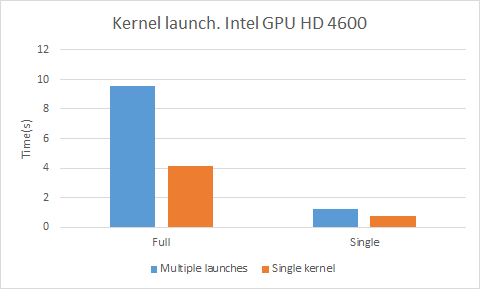
\includegraphics{IntelKernelLaunch}
	\caption{Showing the execution time of a convolutional layer using a single kernel and multiple kernel launches. Full means a fully connected convolutional layer with 4 inputs and 8 outputs. Single means single connections between 4 inputs and 4 outputs}
	\label{fig:intelGPUKernelLaunch}
\end{figure}
\begin{figure}[H]
	\centering
	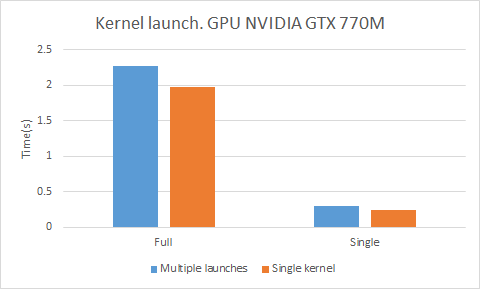
\includegraphics{NvidiaGPUKernelLaunch}
	\caption{Showing the execution time of a convolutional layer using a single kernel and multiple kernel launches. Full means a fully connected convolutional layer with 4 inputs and 8 outputs. Single means single connections between 4 inputs and 4 outputs}
	\label{fig:nvidiaGPUKernelLaunch}
\end{figure}
\begin{figure}[H]
	\centering
	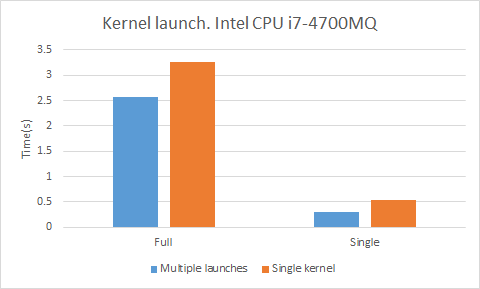
\includegraphics{IntelCPUKernelLaunch}
	\caption{Showing the execution time of a convolutional layer using a single kernel and multiple kernel launches. Full means a fully connected convolutional layer with 4 inputs and 8 outputs. Single means single connections between 4 inputs and 4 outputs}
	\label{fig:cpuKernelLaunch}
\end{figure}

Figure \ref{fig:intelGPUKernelLaunch} and \ref{fig:nvidiaGPUKernelLaunch} looks natural since our intuition says that a kernel launch is expensive. It's important to note here that we don't sum the outputs from the multiple launches which is done in the single full kernel launch. So the full single kernel is actually more expensive than the multiple kernel launches. However, we can see something interesting when looking at Figure \ref{fig:cpuKernelLaunch}. Here multiple kernel launches seems actually more efficient than performing a single one. It could be argued that the kernel launch overhead is almost insignificant when using the CPU and the reduced amount of work becomes significant. Since the same kernel with the same arguments and memory is launched several times, it could also be that the OpenCL runtime notice this and can save significant initialization costs.

  \begin{itemize}
  	\item  The GPU does not have fancy branch prediction and smart caches so this must be handled manually.
  	\item Small loops can degrade performance. Unrolling them can in some cases improve performance.
	\item Local memory does not automatically improve the performance of the GPU. The overhead of putting global memory into local memory has to be small in comparison with the performance gains.
	\item The local work size can have a significant impact. Especially in the case where local memory is used since it will be bound to the work size.
	\item The GPU is more sensitive to kernel launches than the CPU.
  \end{itemize}
  
There are also other pitfalls one have to take into account when writing fast OpenCL code. For example, if you run OpenCL on the host (the CPU), then use calls to clEnqueueMapBuffer and clEnqueueUnmapBuffer instead of calls to clEnqueueReadBuffer or clEnqueueWriteBuffer. This will avoid unnecessary copying within the framework.
  
\section{Automatically tuned OpenCL kernels}

For a CPU, we don't care about local memory. For a GPU, we don't try batch computations in the work items since the scheduling is efficiently done. The general approach to all tuning is to define a default kernel for the CPU and GPU that will represent the benchmark for the problem. If automatic tuning is chosen, the algorithm will try to choose the fastest kernel among the modifiable parameters for the problem. This is typically testing the native / preferred vectorization width of the device and modifying the local work size together with the L1 cache size. Let us start with some notations for this chapter.

\begin{table}[H]
	\centering
	\begin{tabular}{|l| l|}
		\hline
		$U$ & Number of parallel processing units.\\
		\hline
		$S_x, S_y, S_z$ & The problem size dimensions \\
		\hline
		$T_{max}$ & Maximum amounts of threads $T_{max} \geq U$ \\
		\hline
		$S_{l,x}, S_{l,y}, S_{l,z}$ & The local work group dimensions \\
		\hline
		$H_{image}, W_{image}, N_{image}$ & Image height, width and number of images\\
		\hline
		$F_{x}, F_{y}, N_{filter}$ & Filter height and width and the number of filters\\
		\hline
	\end{tabular}
	\caption{Fundamental weighed sub-sampling equations.}
\end{table}

\subsection{Convolutional layer}
\subsubsection{CPU}

\subsubsection{GPU}
There's a big difference between a benchmark CPU kernel and a GPU kernel. In this case, we don't want to have thread affinity for the amount of processing units, which in turn contains a considerable amount of ALUs sharing the same decoder. If we were to have thread affinity for the GPU, we would only use a fraction of the power of the GPU (actually 1 divided by the amount of ALUs in every stream processor, assuming a naive architecture and compiler of course). Instead, since we don't have any scheduling overhead (for what I've detected so far), we simply have one work item for every pixel in the input. However, the focus here will lie in using local memory to speed up memory access. What we know at the moment is:
\begin{itemize}
	\item Every pixel from the input must be read at least once in order for the convolution to work.
	\item But, the local memory is limited to a single local work group. The amount of memory that we can store in the cache is thus dependent on the local work group.
	\item We have boundaries that needs to be treated separately when performing convolution.
	\item The global memory accesses of the output map cannot be smaller than the amount of pixels in the output.
	\item The filters can be loaded into every cache on every streaming processor. However, this will reduce the amount of available local memory for the actual convolution and should be taken into account.
\end{itemize}
To formula for the number of global memory accesses needed for a naive convolution is given by:
\begin{gather*}
S_z(S_x - R_x)(S_y - R_y)F_xF_y\\
R_x = F_x + 1\\
R_y = F_y + 1\\
\end{gather*}
And if we load the work group size together with the boundaries into local memory, we have:
\begin{equation*}
S_z(S_x - R_x)(S_y - R_y) + S_{l,z}(S_x - R_x)(S_y - R_y) ( \frac{R_x}{S_{l,x}} + \frac{R_y}{S_{l,y}} + \frac{R_xR_y}{S_{l,x}S_{l,y}} + 1)
\end{equation*}
We can directly see that the amount of global memory accesses decreases dramatically for a big local size in the x and y directions. However, we need to be careful with the conclusions here since we have additional complexity when choosing the local work group size.
\begin{itemize}
	\item The local work group executes in parallel on a stream processor. Meaning that, if our local work group is as big as the problem itself, we cannot benefit from the parallel execution of several streaming processors.
	\item The filters will have as many memory accesses as the naive equation. A very simple way to make sure we don't access global memory for the filters is to put them onto the constant memory by using the constant modifier.
	\item The local work size should therefore be considered as the maximum local work size that can be distributed on all the streaming processors (as long as the filter is not equal to one). The second constraint is that the amount of local memory cannot be exceeded and this must be queried on the kernel. 
\end{itemize}
We have additional constrains when defining the local memory size and using the constant memory.
\begin{itemize}
	\item The local cache size cannot exceed the value returned by  CL\_DEVICE\_LOCAL\_MEM\_SIZE - CL\_KERNEL\_LOCAL\_MEM\_SIZE before setting the cache size.
	\item The local work size cannot exceed CL\_KERNEL\_WORK\_GROUP\_SIZE.
	\item The filter parameters used for the convolution cannot exceed \\ CL\_DEVICE\_MAX\_CONSTANT\_BUFFER\_SIZE if we are to use the constant memory space for the parameters. The minimum value is 64KB, which corresponds to 16 000 parameters. In turn, 16 000 parameters would correspond to about 55 21x21 filters in a single layer. This would only be a problem for extremely large problems. In this case, it would be acceptable to split the problem into two kernel calls (or more).
\end{itemize}
Since a greater value on $S_{l,z}$ than 1 will always increase the amount of global memory accesses. We will always assume that $S_{l,z} = 1$. Furthermore, we will always assume that the filter is in constant memory space. This leads to the following discrete constrained optimization problem for reducing the amount of global memory accesses:
\begin{gather*}
(S_{l,x}, S_{l,y})_{min} = \min_{(S_{l,x}, S_{l,y})} S_z(S_x - R_x)(S_y - R_y) + \\
 \frac{(S_x - R_x)(S_y - R_y)}{S_{l,x}S_{l,y}} ( R_xS_{l,y} + R_yS_{l,x} + R_xR_y + S_{l,x}S_{l,y}) \\
(S_x - R_x) \mod{S_{l,x}} \equiv 0 \\
(S_y - R_y) \mod{S_{l,y}} \equiv 0 \\
S_{l,x} \leq S_{l,x, max} \\
S_{l,y} \leq S_{l,y, max} \\
 \frac{(S_x - R_x)(S_y - R_y)}{S_{l,x}S_{l,y}} \geq U \\
S_{l,y}S_{l,x} \leq CL\_KERNEL\_WORK\_GROUP\_SIZE \\
R_x S_{l,y} + R_y S_{l,x} + R_xR_y + S_{l,y}S_{l,x} \leq M \\
M = CL\_DEVICE\_LOCAL\_MEM\_SIZE - CL\_KERNEL\_LOCAL\_MEM\_SIZE
\end{gather*}
However, as you can see, it's possible that the conditions that the local work group must be dividable with the global work group will not hold. In this case we need to transform the above optimization problem with padding to make sure that it may be solved.
\begin{gather*}
(S_{l,x}, S_{l,y}, P_x, P_y)_{min} = \min_{(S_{l,x}, S_{l,y}, P_x, P_y)} S_z(S_x + P_x - R_x)(S_y + P_y - R_y) + \\
\frac{(S_x + P_x - R_x)(S_y + P_y - R_y)}{S_{l,x}S_{l,y}} ( R_xS_{l,y} + R_yS_{l,x} + R_xR_y + S_{l,x}S_{l,y}) \\
(S_x + P_x - R_x) \mod{S_{l,x}} \equiv 0 \\
(S_y  + P_y - R_y) \mod{S_{l,y}} \equiv 0 \\
S_{l,x} \leq S_{l,x, max} \\
S_{l,y} \leq S_{l,y, max} \\
\frac{(S_x + P_x - R_x)(S_y + P_y - R_y)}{S_{l,x}S_{l,y}} \geq U \\
S_{l,y}S_{l,x} \leq CL\_KERNEL\_WORK\_GROUP\_SIZE \\
R_x S_{l,y} + R_y S_{l,x} + R_xR_y + S_{l,y}S_{l,x} \leq M \\
M = CL\_DEVICE\_LOCAL\_MEM\_SIZE - CL\_KERNEL\_LOCAL\_MEM\_SIZE
\end{gather*}
The solution to the above optimization problem is given by: \\
\begin{algorithm}[H]
	\DontPrintSemicolon
	OptimalLocalSize\;
	\KwData{Kernel, Device}
	\KwResult{$(S_{l,x}, S_{l,y}, P_x, P_y)_{min}$}
	Hypotheses \;
	\For {$P_x$ : from 0 to $S_{l,x, max}$}
	{
		\For {$P_y$ : from 0 to $S_{l,y, max}$}
		{
				\For {$S_{l,x}$ : from 0 to $S_{l,x, max}$}
				{
					\For {$S_{l,y}$ : from 0 to $S_{l,y, max}$}
					{
					\If{$(S_x + P_x - R_x) \mod{S_{l,x}} \not\equiv 0$ or \; $(S_y  + P_y - R_y) \mod{S_{l,y}} \not\equiv 0$ or $S_{l,y}S_{l,x} > CL\_KERNEL\_WORK\_GROUP\_SIZE$ or
						$\frac{(S_x + P_x - R_x)(S_y + P_y - R_y)}{S_{l,x}S_{l,y}} < U$ or
						$R_x S_{l,y} + R_y S_{l,x} + R_xR_y + S_{l,y}S_{l,x} > M $\;}
					{
						continue\;
					}
					\Else
					{
						Hypotheses.add($(S_{l,x}, S_{l,y}, P_x, P_y)$);
					}
				}
			}
		}
	}
	$min = \infty$ \;
	\For{Hypothesis in Hypotheses}
	{
		$accesses = S_z(S_x + P_x - R_x)(S_y + P_y - R_y) +
		\frac{(S_x + P_x - R_x)(S_y + P_y - R_y)}{S_{l,x}S_{l,y}} ( R_xS_{l,y} + R_yS_{l,x} + R_xR_y + S_{l,x}S_{l,y})$ \;
		\If{$min < accesses$}
		{
		$(S_{l,x}, S_{l,y}, P_x, P_y)_{min}$ = $(S_{l,x}, S_{l,y}, P_x, P_y)$ \;
			$min = accesses$
		}
	}
\caption{Calculates the optimal work size and padding with minimal global memory access.}
\end{algorithm}
The above implementation is very naive and one should probably limit the padding to a fixed value of say 10 in order not to explode the computations. A common max value on the work dimension is around 1000 and by using this naive approach it could take way too long to calculate the benchmark kernel.
\begingroup
\huge ADD TUNING
\endgroup 
\subsection{Pooling layer}
\subsubsection{CPU}
\subsubsection{GPU}
\subsection{Perceptron layer} 
\subsubsection{CPU}
\subsubsection{GPU}
\bibliography{sample}

\appendix

\end{document}
